\documentclass[onecolumn, draftclsnofoot, 10pt, compsoc]{IEEEtran}
\usepackage{graphicx}
\graphicspath{{./figures/}}

\usepackage{url}
\usepackage{setspace}
\usepackage{multicol}
\usepackage{pdflscape}
\usepackage{pdfpages}
\usepackage[british]{babel}
\usepackage{listings}
\usepackage{xcolor}
\usepackage{listings}
\usepackage{hyperref}
\usepackage{subfig}
\usepackage{pdfpages}
\usepackage{longtable}

\usepackage{geometry}
\geometry{textheight=9.5in, textwidth=7in}

\hypersetup{
    colorlinks=true,
    linkcolor=blue,
    filecolor=magenta,      
    urlcolor=cyan,
}

% \overfullrule=2in

% 1. Fill in these details
\def \CapstoneTeamName{			Ground Station Software Team}
\def \CapstoneTeamNumber{		30}
\def \GroupMemberOne{			Kenneth Steinfeldt}
\def \GroupMemberTwo{			Christopher Pham}
\def \GroupMemberThree{			Corwin Perren}
\def \CapstoneProjectName{		OSU Robotics Club\\Mars Rover Ground Station}
\def \CapstoneSponsorCompany{	OSU Robotics Club}
\def \CapstoneSponsorPerson{	Nick McComb}



%Personal \newcommands

\newcommand{\functRequ}[4]{
\item #1%
\par
\begin{itemize}
\item \textit{Description:} #2.%
\item \textit{Rationale:} #3.%
\item \textit{Dependencies:} #4%
\end{itemize}
}
\definecolor{backcolor}{rgb}{0.95,0.95,0.92}
\lstset{basicstyle=\ttfamily,
  backgroundcolor=\color{backcolor},  
  showstringspaces=false,
  commentstyle=\color{red},
  keywordstyle=\color{blue},
  columns=fullflexible,
  breaklines=true,
  postbreak=\mbox{\textcolor{red}{$\hookrightarrow$}\space},
}


% 2. Uncomment the appropriate line below so that the document type works
\def \DocType{	%Problem Statement
				%Requirements Document
				%Technology Review
				%Design Document
				Final Report
			 }
			
\newcommand{\NameSigPair}[1]{
  \par
  \makebox[2.75in][r]{#1} 
  \hfill
  \makebox[3.25in]{
      \makebox[2.25in]{\hrulefill} 
      \hfill
      \makebox[.75in]{\hrulefill}
  }
  \par\vspace{-12pt} 
  \textit{
      \tiny\noindent
      \makebox[2.75in]{} 
      \hfill
      \makebox[3.25in]{
          \makebox[2.25in][r]{Signature} 
          \hfill
          \makebox[.75in][r]{Date}
      }
  }
}
% 3. If the document is not to be signed, uncomment the command below
\renewcommand{\NameSigPair}[1]{#1}

%%%%%%%%%%%%%%%%%%%%%%%%%%%%%%%%%%%%%%%
\begin{document}
\begin{titlepage}
	\pagenumbering{gobble}
	\begin{singlespace}
		% 4. If you have a logo, use this includegraphics command to put it on the coversheet.
        \begin{minipage}{7in}
			\centering
			\hspace*{-.7in}
			$\vcenter{\hbox{
\includegraphics[height=4cm]{Oregon_State_College_of_Engineering_Logo}}}$
			\hspace*{.2in}
			$\vcenter{\hbox{
\includegraphics[height=2.5cm]{OSURCLogoOrange}}}$
		\end{minipage}

		\par\vspace{.35in}
		\centering
		\scshape{
			\huge CS Capstone \DocType \par
			{\large\today}\par
			\vspace{.5in}
			\textbf{\Huge\CapstoneProjectName}\par
			\vfill
			{\large Prepared for}\par
			\Huge \CapstoneSponsorCompany\par
			\vspace{5pt}
			{\Large\NameSigPair{\CapstoneSponsorPerson}\par}
			{\large Prepared by }\par
			Group\CapstoneTeamNumber\par
			% 5. comment out the line below this one if you do not wish to name your team
			\CapstoneTeamName\par 
			\vspace{5pt}
			{\Large
				\NameSigPair{\GroupMemberOne}\par
				\NameSigPair{\GroupMemberTwo}\par
				\NameSigPair{\GroupMemberThree}\par
			}
			\vspace{20pt}
            \begin{abstract}
			% 6. Fill in your abstract
			This document contains all of the useful documentation about the OSURC Mars Rover ground station project as it has progressed throughout the year. This includes all technical documents (with revisions), weekly blog posts, code documentation, and lessons learned.

		\end{abstract}
		}
	\end{singlespace}
\end{titlepage}
\newpage
\pagenumbering{arabic}
\tableofcontents
\clearpage

% Write stuff here....
\section{Introduction}
\subsection{Who Requested the Project?}
This project was requested by the Oregon State University Robotics Club's (OSURC) Mars Rover team.

\subsection{Why Was the Project Requested?}
This project was requested due to the Mars Rover team's need for a complete and functional ground station in a time frame that the existing software team may not have been able to accomplish. Additionally, new requirements for the ground station meant that the increased complexity was most likely going to require a more dedicated team to complete than the volunteers the club normally has working on the Mars Rover project.

\subsection{What is the Importance of the Project?}
This project solves some of the most common problems for the Mars Rover team in previous competition years. Historically, the team is allowed a 10-15 minute set up time during competition where the Rover must be turned on, ground station connected, and core systems tested before actually competing in a task. In previous years, the Rover's ground station has normally been a laptop with a handful of random pieces of hardware plugged into it over USB. Many times, this hardware has been damaged during transit and caused problems during the setup phase. Additionally, previous software has often been command line driven and extremely specialized meaning the software is difficult to use, difficult to teach, and has ended up getting re-written with each new Rover competition year.

\subsection{Our Client and Their Role}
Our client was Nick McComb, team lead and electrical lead of the Mars Rover team for the 2017-2018 competition year. His role was mainly supervisory, helping our group set up the initial requirements for the software, and occasionally making requests for additional features as the year progressed. 

\subsection{Our Team Members and Roles}
\begin{itemize}
\item Chris Pham
	\begin{itemize}
    \item Rover mapping systems
	\end{itemize}
\item Ken Steinfeldt
	\begin{itemize}
    \item Rover status systems
	\end{itemize}
\item Corwin Perren
	\begin{itemize}
	\item Team Manager
    \item Rover video systems
    \item Program structure / startup
	\end{itemize}
\end{itemize}

\section{Requirements Document}
\subsection{Original Document}
\includepdf[pages=-, frame=true, scale=0.95]{02-requirementsdoc/group-design-requirements.pdf}

\subsection{Additions}
\subsubsection{Final Revision Document}
\includepdf[pages=-, frame=true, scale=0.95]{02-requirementsdoc/cs_group30_design_requirements_revision1_1.pdf}

\subsubsection{Description of Changes}
Version 1.1 of document was approved by all team members and stakeholder on 4/26/2018.

\begin{itemize}
\item Edited descriptions of competition from University Rover Challenge to Canadian International Rover Challenge
	\begin{itemize}
	\item The Mars Rover team changed competitions, so we updated the document to reflect this
	\end{itemize}
    
\item Removed user story for manual video quality adjustment
	\begin{itemize}
	\item Our team implemented automatic quality adjustment, so manual adjustment was no longer necessary
	\end{itemize}
    
\item Removed user story about easily seeing when an autonomous run has completed
	\begin{itemize}
	\item The new Rover competition does not require this display element
	\end{itemize}
    
\item Removed user story about needing to view live logs
	\begin{itemize}
	\item Log viewing was determined to not be needed as there would be too many logs to sort through in a short amount of time
	\end{itemize}
    
\item Removed user story about seeing network latency (round trip time)
	\begin{itemize}
	\item The network connection percentage was determined to be correlated with this value enough that this redundant element was not needed
	\end{itemize}

\item Added constraint that the GUI software must have placeholder for GUI elements and software features that can not be completed due to waiting on Rover team progress
	\begin{itemize}
	\item Our team encountered many situations where we could not continue development due to lack of hardware/software on Rover
    \item This new constraint allows us to still meet requirements if the bottleneck is the Rover team
	\end{itemize}
    
\item Changed functional requirement for joystick statuses so that the SpaceNav mouse had its own requirement
	\begin{itemize}
	\item The team changed to a SpaceNav mouse earlier in the year and it was determined that an individual readout for this input device would be convenient
	\end{itemize}
    
\item Changed functional requirement for battery status to battery voltage
	\begin{itemize}
	\item The battery status value was determined to be most useful as a voltage, rather than a percentage estimate
	\end{itemize}
    
\item Removed functional requirement for Rover voltage statuses
	\begin{itemize}
	\item The Rover design changed so that only the battery voltage is measured
	\end{itemize}
    
\item Changed functional requirement for bogie connection statuses to be individual wheel statuses
	\begin{itemize}
	\item The Rover software team got individual status information for each wheel, rather than a two wheel bogie group, and requested this change
	\end{itemize}
    
\item Removed functional requirement for Rover network round trip time
	\begin{itemize}
	\item The network connection percentage was determined to be correlated with this value enough that this redundant element was not needed
	\end{itemize}
    
\item Changed functional requirement for Rover arm joystick control to SpaceNav mouse control
	\begin{itemize}
	\item The team changed to a SpaceNav mouse over a second joystick for arm control
	\end{itemize}
    
\item Removed functional requirement for way-point navigation path
	\begin{itemize}
	\item Expectations for how autonomy on the Rover would work would not easily give our team this information to display
	\end{itemize}
    
\item Changed functional requirement for the autonomy indicator so that it shows whether autonomy is active rather than when autonomy is finished
	\begin{itemize}
	\item Changing to the Canadian International Rover Challenge made the old requirement unnecessary
	\end{itemize}
    
\item Removed functional requirement for video FPS counters
	\begin{itemize}
	\item FPS counters would have been useful for manual video quality adjustment, but are no longer needed with automatic quality adjustment
	\end{itemize}
    
\item Removed functional requirement for log file viewing
	\begin{itemize}
	\item Log files were too large to usefully sort through in a short amount of time
	\end{itemize}
    
\end{itemize}

\subsection{Final Gantt Chart}
\includepdf[pages=-, frame=true, landscape, scale=0.95]{02-requirementsdoc/final_gantt.pdf}
\section{Design Document}
\subsection{Original Document}
\includepdf[pages=-, frame=true, scale=0.95]{03-designdoc/group-design-document.pdf}
\subsection{Additions}
There were no additions to our original design document.
\section{Tech Review Document}
\subsection{Original Documents}
\subsection{Chris Pham}
\subsubsection{Week 1}
This first week of classes for the three of us was mostly planning on what to exactly doing for the next 10 weeks and what exactly our working times are.
We planned for Tuesdays, Thursdays, and Saturdays because that's when Ken is supposed to be down and everyone seems to be free on those days.
Another thing that did come up was that the expectation that we should go to the OSU Robotics Club's Mars Rover Meetings on Saturday at 12 in the afternoon.
Another bonus of Saturday's is that that is when the team has working hours and we can interact with the people creating the systems on the rover side.
After deciding our times, we decided on who should do what task using our Asana and dictated by the club and our client.
It was decided that I would be doing Mapping and the others doing video and connection statuses.
\\
I was first prototyping using the Google Maps Static API and Python 2.7 to grab the tile at the given GPS location.
It worked, but I ended up thinking about how to stitch this object correctly.
I was also contemplating zooming in on the image instead of using stitching to remove complexity.
I do not have my code now from testing out the API because I reformatted this computer completely to install the requirements for the project, Ubuntu 16.04 and more importantly ROS.
\subsubsection{Week 2}
On Saturday, I started working on trying to search how to stitch images using Google Images.
I was told that last year they used this class package called GooMPy that took care of that for them and I spent my time looking at this code and trying to understand what it does.
We also took a group photo and I was introduced to the software team of the Rover.
It turned out they're mostly Freshman and they did not finish their Python reviews yet, so they could not start on the rover software that we need to interact with.
\\
On Tuesday, we met up in our club room and did some basic things with Qt Designer so we would be caught up on designing that.
I had some questions about some things like the API calling limit we have for Google Maps, and it turns out we will almost never hit the API limit.
Another thing was multi-threaded performance because how this file worked was that it did a bunch of Google Maps calls and then merged them with PIL (Python Image Library) and this looked doable to multi-thread.
However, one issue we have is the effect of Qt's QThreads and the multi-threading process for Python playing nicely with each other.
After talking about that, I then made created a branch in git and then built my files based upon GooMPy and made it more class based so it makes more sense for grouping and private variables.
The troubles with the structured format of the old file makes it hard to understand with the lack of comments and weird structures that is not expected in Python. 
All progress during this week was during January 18, 2018:\\
\begin{center}
\begin{tabular}{l l l l}	\textbf{Detail} & \textbf{Author} & \textbf{Date} &\textbf{Description}\\\hline
\href{https://github.com/OSURoboticsClub/Rover_2017_2018/commit/bb8ed586e278eaa18b1861a0949afa53a743c876}{bb8ed58} & Chris Pham & 2018-01-18 10:37:41 -0800 &Make Mapping Core (mapping.py)\\\hline
\href{https://github.com/OSURoboticsClub/Rover_2017_2018/commit/47942ffd1dcc2b3a1e29776d00a005f5a4247ea3}{47942ff} & Chris Pham & 2018-01-18 10:40:47 -0800 &Added Imports\\\hline
\href{https://github.com/OSURoboticsClub/Rover_2017_2018/commit/c8c8f857cd2de7d01a5c790a22ac643a6b962436}{c8c8f85} & Chris Pham & 2018-01-18 10:47:56 -0800 &Add Constants\\\hline
\href{https://github.com/OSURoboticsClub/Rover_2017_2018/commit/a9f36af40d4c3a00bb2336852d0db329f3b5905e}{a9f36af} & Chris Pham & 2018-01-18 10:53:39 -0800 &Read key from file\\\hline
\href{https://github.com/OSURoboticsClub/Rover_2017_2018/commit/7e593097eab330b71a54b56251a1bea11e31a72c}{7e59309} & Chris Pham & 2018-01-18 10:55:42 -0800 &Made apikey file, and fixed open error\\\hline
\href{https://github.com/OSURoboticsClub/Rover_2017_2018/commit/b82a39d3bf666abd8ed38839d6c5730b09e6ad04}{b82a39d} & Chris Pham & 2018-01-18 10:58:24 -0800 &fixed fp naming conventions\\\hline
\href{https://github.com/OSURoboticsClub/Rover_2017_2018/commit/3570c4b5735bc2dbdf39bb5f52d34ccaa5bbee7e}{3570c4b} & Chris Pham & 2018-01-18 11:09:09 -0800 &write file intro\\\hline
\href{https://github.com/OSURoboticsClub/Rover_2017_2018/commit/a9bf793bfc0db615d7d62bef7ac1d56f81c38d6c}{a9bf793} & Chris Pham & 2018-01-18 11:21:05 -0800 &add gmaps obj and init\\\hline
\href{https://github.com/OSURoboticsClub/Rover_2017_2018/commit/c2bb5f6d31e6457d59e207c5f87edeeb2ac50e11}{c2bb5f6} & Chris Pham & 2018-01-18 12:14:06 -0800 &Added pixel\_to\_degrees helper\\\hline
\href{https://github.com/OSURoboticsClub/Rover_2017_2018/commit/f203cee53e0a60c4dc8eed40dfae0a07e4649e59}{f203cee} & Chris Pham & 2018-01-18 12:24:01 -0800 &rebuild Google Maps API link\\\hline
\href{https://github.com/OSURoboticsClub/Rover_2017_2018/commit/d09dbb1a02bc8883bc16e68aa8de74ee1b6ecfe6}{d09dbb1} & Chris Pham & 2018-01-18 12:43:03 -0800 &Addded \_grab\_tile helper\\\hline
\href{https://github.com/OSURoboticsClub/Rover_2017_2018/commit/16f76fad49699b346e15c0fdcfc2edcb814a0123}{16f76fa} & Chris Pham & 2018-01-18 13:00:53 -0800 &added \_pixels\_to\_lon helper\\\hline
\href{https://github.com/OSURoboticsClub/Rover_2017_2018/commit/b7348ee897a3bbff349d2d04d7c2084bc60c46f0}{b7348ee} & Chris Pham & 2018-01-18 13:07:21 -0800 &Fix self in pixel\_to\_lon helper\\\hline
\href{https://github.com/OSURoboticsClub/Rover_2017_2018/commit/400410cea4af92cb25fd1f686809f320c9cc102c}{400410c} & Chris Pham & 2018-01-18 13:21:38 -0800 &Added \_pixels\_to\_lat\\\hline
\href{https://github.com/OSURoboticsClub/Rover_2017_2018/commit/d2f4fc38fecf903ed35d731dafe566709707601c}{d2f4fc3} & Chris Pham & 2018-01-18 13:23:48 -0800 &Add gitignore for API key\\\hline
\href{https://github.com/OSURoboticsClub/Rover_2017_2018/commit/b319118e1d32c8d655afe7a6cd084916d16f8db3}{b319118} & Chris Pham & 2018-01-18 13:26:03 -0800 &remove key\\\hline
\end{tabular}
\end{center}
\subsubsection{Week 3}
During the meeting on Saturday, I was informed that there is a API key and signature that I should use so I don't get throttled nor limited on calls.
I was finishing up some of my helper functions for my class object and then fixed my code to fit PEP8 conventions.
Then to implement my code, I made a new file called sign.py to take in a string and then return me the correct signature to append to the string for Google to accept.
Once that was done, I built a testing script to call the object and then save the big image somewhere on my computer.
Turns out my laptop hates that and I froze my computer for 20 minutes and once that was done, I edited the .gitignore to ignore the .jpg files I was downloading from the API.
\\
On Thursday, I was trying to get my zooming to work correctly on this image, but I can't do it from the API and I would have to do it from Qt or from OpenGL.
I also made a smaller display image to display it onto the display space on the GUI and for my computer to run.
\begin{center}
\begin{tabular}{l l l l}
\textbf{Detail} & \textbf{Author} & \textbf{Date} &\textbf{Description}\\\hline
\href{https://github.com/OSURoboticsClub/Rover_2017_2018/commit/995386ee89319296165900b1466b6cfc5cf060d5}{995386e} & Chris Pham & 2018-01-20 13:06:28 -0800 &Made pixels\_to\_meters helper\\\hline
\href{https://github.com/OSURoboticsClub/Rover_2017_2018/commit/fee5b5537bbdb496791f7b7f323aae6995844afc}{fee5b55} & Chris Pham & 2018-01-20 13:24:32 -0800 &Added logic for num\_sqares\\\hline
\href{https://github.com/OSURoboticsClub/Rover_2017_2018/commit/3565e7b57f1f19a81b9b34b88a8c9ef527e7c7d6}{3565e7b} & Chris Pham & 2018-01-20 13:43:47 -0800 &Rebuild grab\_tile\\\hline
\href{https://github.com/OSURoboticsClub/Rover_2017_2018/commit/e955442131978ffd1d24aa6ced9ff2c9f899ed59}{e955442} & Chris Pham & 2018-01-20 13:57:11 -0800 &Fixed to fit PEP\\\hline
\href{https://github.com/OSURoboticsClub/Rover_2017_2018/commit/332c751758c837cb52b3a9008ba830c5755fbf76}{332c751} & Chris Pham & 2018-01-20 14:14:44 -0800 &Append signature\\\hline
\href{https://github.com/OSURoboticsClub/Rover_2017_2018/commit/a0601abb8db35bf4a7ebcdba81f702814c73fdf2}{a0601ab} & Chris Pham & 2018-01-20 16:32:58 -0800 &Add testing file with updated gitignore for jpgs\\\hline
\href{https://github.com/OSURoboticsClub/Rover_2017_2018/commit/1c16cb48a1faec2e8dc157748d0f870d1253fde7}{1c16cb4} & Chris Pham & 2018-01-25 10:49:36 -0800 &Creates Big Image\\\hline
\href{https://github.com/OSURoboticsClub/Rover_2017_2018/commit/b12f8fc986912d75d018e8da9912eaa1c93b9e4b}{b12f8fc} & Chris Pham & 2018-01-25 15:01:35 -0800 &Working updates and fetching, starting on zoom functionality\\\hline
\end{tabular}
\end{center}
\subsubsection{Week 4}
This week, I had a bunch of troubles trying to get most of my stuff working correctly.
One big issue with my code was the latitude and longitude values to pixel coordinates. For some reason my values would be pointing to the wrong locations.
From the research I did about this issue, I can explain better why these equations are used at least.
I spent around 4 hours working on this and I had to leave to do something else on the side.
\\
I was thinking it could be the skew from the center of the map towards the outsides compared to just getting the outside values at the start.
I tried to get the boundaries when generating map and then cutting the value in half to get the approximate centering.
That did not work at all and I just gave up on it for a bit and went ahead and tried to program something else like putting icons on the map correctly.
Somehow, when I copied the code from the previous function, and then used it, it provided the correct locations and I was really confused.
Then I used the function that I just made and used that to center my map to see if that worked and it did.
Once I got that part working, I then made some way of adding icons to the image to quickly prototype my way-point system.
Here are some examples of my code via images, before and after:
\begin{figure}[ht!]
\begin{minipage}[t]{.45\linewidth}\centering
\includegraphics[width=\linewidth]{figures/unzoomed}
\caption{Before, Centered at Kelly}
\end{minipage}\hfill
\begin{minipage}[t]{.45\linewidth}\centering
\includegraphics[width=\linewidth]{figures/centered}
\caption{After, Centered at Kelly and points at MU and Valley}
\end{minipage}
\end{figure}
\newline
One of the next issues I thought about was trying to reduce computation time and I was thinking of using a way-point later to control and manage any drawing on the screen.
I can make a transparent layer/image with alpha levels with icons I can inject via PIL that I can draw each time instead of using disk time to get the images again
That can be done using Qt I think, or even PIL can do it, but it might take a hit on computation times.
\begin{center}
\begin{tabular}{l l l l}	\textbf{Detail} & \textbf{Author} & \textbf{Date} &\textbf{Description}\\\hline
\href{https://github.com/OSURoboticsClub/Rover_2017_2018/commit/3ed2c5977e41dc8f4baee7b10d7c3114793e29d7}{3ed2c59} & Chris Pham & 2018-02-01 19:25:54 -0800 &created and fixed centering\\\hline
\href{https://github.com/OSURoboticsClub/Rover_2017_2018/commit/5f12d8074f8fcfb799f6ac3493cb39081bb7f7c3}{5f12d80} & Chris Pham & 2018-02-01 19:55:57 -0800 &starting on map updatiing\\\hline
\href{https://github.com/OSURoboticsClub/Rover_2017_2018/commit/75adf70d5bfba0e4b7b48bf7cefbc88feb68f4de}{75adf70} & Chris Pham & 2018-02-02 11:30:16 -0800 &define \_\_str\_\_\\\hline
\href{https://github.com/OSURoboticsClub/Rover_2017_2018/commit/d012360da50b074efb9a1cc1f7c1e0dacda207e7}{d012360} & Chris Pham & 2018-02-02 13:11:06 -0800 &remove prints\\\hline
\hline\end{tabular}
\end{center}
\subsubsection{Week 5}
This week was building and refactoring my object class so it had a helper class to do work for it too.
I rearranged it because I needed to use some of those function myself for building the way-point overlay system I going to implement for my system.
On Saturday, I merged my branch into the Master, but that took a bit of time because I had to rebase my branch into fitting the current master branch.
Once it was rebased to fit the master branch, I then had to do some 'git mv' to move some files around go the correct locations.
Once that was finished, I could finish my pull request and I could go on with some other tasks.
I started commenting and documenting my progress using docstrings and then applying PEP8 standard for the rest of my code, which meant that I needed to decrease the amount of characters were on a line most of the time.
After finishing up all of that, I started on making the coordinator between the class and the QObject that I needed to use to get Qt to work correctly with this object.
\begin{center}
\begin{tabular}{l l l l}\textbf{Detail} & \textbf{Author} & \textbf{Date} & \textbf{Description}\\\hline
\href{https://github.com/OSURoboticsClub/Rover_2017_2018/commit/15154f912ff4204e8a3bcf48299592d1fb8bc2ca}{15154f9} & Chris Pham & 2018-02-03 12:49:43 -0800 &Merge branch 'Mapping\_Core' of https://github.com/OSURoboticsClub/Rover\_2017\_2018 into Mapping\_Core\\\hline
\href{https://github.com/OSURoboticsClub/Rover_2017_2018/commit/07534f8487ba8a04d63e73c22385158479c3c6cc}{07534f8} & Chris Pham & 2018-02-03 13:45:51 -0800 &Starting of mapping class refactor\\\hline
\href{https://github.com/OSURoboticsClub/Rover_2017_2018/commit/06c605ebd5780e65f1f7ad077ef5cf7a136d2a18}{06c605e} & Chris Pham & 2018-02-03 13:46:46 -0800 &remove idea file\\\hline
\href{https://github.com/OSURoboticsClub/Rover_2017_2018/commit/e65d4e5067d4b3f9b1223a57f7666131e2c2cf6f}{e65d4e5} & Chris Pham & 2018-02-03 13:50:32 -0800 &Move new\_image function to helper\\\hline
\href{https://github.com/OSURoboticsClub/Rover_2017_2018/commit/37303e3a95020e41aadea474e2d6e95c543f5af0}{37303e3} & Chris Pham & 2018-02-03 13:53:21 -0800 &Moved fast\_round to helper\\\hline
\href{https://github.com/OSURoboticsClub/Rover_2017_2018/commit/0cbd593380d86ca3d479b7e40167273641c8c04d}{0cbd593} & Chris Pham & 2018-02-03 13:56:15 -0800 &Add pixels\_to\_degrees to helper\\\hline
\href{https://github.com/OSURoboticsClub/Rover_2017_2018/commit/10c9dc8451a582e67e8475e2bf161054191f1d02}{10c9dc8} & Chris Pham & 2018-02-03 14:02:23 -0800 &Make static functions and self reference for helper\\\hline
\href{https://github.com/OSURoboticsClub/Rover_2017_2018/commit/4a66dbc0b5954672d4377a1c9e07c53ccd1d7323}{4a66dbc} & Chris Pham & 2018-02-03 14:06:46 -0800 &Moved pixels\_to\_meters to Helper\\\hline
\href{https://github.com/OSURoboticsClub/Rover_2017_2018/commit/d17aaf5ef8343be017032c46fa391b9b27470bc2}{d17aaf5} & Chris Pham & 2018-02-03 14:37:43 -0800 &Added Docstrings for mapping.py\\\hline
\href{https://github.com/OSURoboticsClub/Rover_2017_2018/commit/b402cd12d3ab294d280cddf85c28ac263f62ce91}{b402cd1} & Chris Pham & 2018-02-03 14:40:46 -0800 &created docstrings for maphelper\\\hline
\href{https://github.com/OSURoboticsClub/Rover_2017_2018/commit/ad51c3d7940eb1c5baa8f4ac0b72fe115c7eb776}{ad51c3d} & Chris Pham & 2018-02-03 14:51:32 -0800 &Finished move\_latlon function\\\hline
\href{https://github.com/OSURoboticsClub/Rover_2017_2018/commit/31ad2185cb708d66cdb29dc23597a8c241622b4f}{31ad218} & Chris Pham & 2018-02-03 14:52:20 -0800 &Comment out waypoints\\\hline
\href{https://github.com/OSURoboticsClub/Rover_2017_2018/commit/23f3554af37f18f17b1ad9c79378f5fc185ebf1a}{23f3554} & Chris Pham & 2018-02-03 15:28:45 -0800 &complying with PEP8 standard\\\hline
\href{https://github.com/OSURoboticsClub/Rover_2017_2018/commit/89e7739f54adcf9317261f4741d1860d9c41a838}{89e7739} & Chris Pham & 2018-02-08 12:58:45 -0800 &Start of RoverMapCoordinator\\\hline
\href{https://github.com/OSURoboticsClub/Rover_2017_2018/commit/33694343176eaedff94334df4083b831ce1bc006}{3369434} & Chris Pham & 2018-02-08 13:33:32 -0800 &Changed file names and started initer for MapCoordinator\\\hline
\href{https://github.com/OSURoboticsClub/Rover_2017_2018/commit/f4d6835e85304f1dd43cea14ac4eb17587b14606}{f4d6835} & Chris Pham & 2018-02-08 13:50:12 -0800 &create label for left xml for map location, and remove \_get\_map.\\\hline
\href{https://github.com/OSURoboticsClub/Rover_2017_2018/commit/4455e5769389aa18ea396a3981cf3a3b989c6271}{4455e57} & Chris Pham & 2018-02-08 13:57:49 -0800 &fixed wrong size references\\\hline
\href{https://github.com/OSURoboticsClub/Rover_2017_2018/commit/cdfc76789173155e7f6fdc8d27137149e6f41fc6}{cdfc767} & Chris Pham & 2018-02-08 14:02:43 -0800 &Corrcted bool and created the thread for the main class\\\hline
\href{https://github.com/OSURoboticsClub/Rover_2017_2018/commit/bb3b47977b1818ff9d45c6144d134e6a34a7d316}{bb3b479} & Chris Pham & 2018-02-08 14:06:12 -0800 &Moved file to software/ground\_station\\\hline
\href{https://github.com/OSURoboticsClub/Rover_2017_2018/commit/e9f03deaa25624aeec6509c72e782cc801fef521}{e9f03de} & Chris Pham & 2018-02-08 14:08:26 -0800 &Merge pull request \#9 from OSURoboticsClub/Mapping\_Core\\\hline
\href{https://github.com/OSURoboticsClub/Rover_2017_2018/commit/f71bcba2b080bbc51f9d5eda2f2ae3010d332f68}{f71bcba} & Chris Pham & 2018-02-08 14:13:53 -0800 &Change the include to correct path and remove test file\\\hline
\href{https://github.com/OSURoboticsClub/Rover_2017_2018/commit/fe53c5d5a73ac253acaef11fef448995f519cca8}{fe53c5d} & Chris Pham & 2018-02-08 14:36:12 -0800 &added init for mapping\\\hline
\href{https://github.com/OSURoboticsClub/Rover_2017_2018/commit/79325aefdf731ab4fcadc9dee58e3359e6c3b289}{79325ae} & Chris Pham & 2018-02-08 14:39:46 -0800 &Added parenthesis\\\hline
\href{https://github.com/OSURoboticsClub/Rover_2017_2018/commit/345c75886dfaf76865e56aedc130ec83f9dd8352}{345c758} & Chris Pham & 2018-02-08 14:40:48 -0800 &remove bang\\\hline
\href{https://github.com/OSURoboticsClub/Rover_2017_2018/commit/8b903d1299d30611ca22aaebc5267e874de4c004}{8b903d1} & Chris Pham & 2018-02-08 14:44:20 -0800 &changed import calls and another bang\\\hline
\href{https://github.com/OSURoboticsClub/Rover_2017_2018/commit/e64c42c45fa51556a9e4e2fba3f2e0450f75a134}{e64c42c} & Chris Pham & 2018-02-08 14:51:35 -0800 &correct super \_\_init\_\_ for map coord\\\hline
\href{https://github.com/OSURoboticsClub/Rover_2017_2018/commit/cba5bc9b39738a42df87b09cea98ffc9599b9617}{cba5bc9} & Chris Pham & 2018-02-08 14:59:56 -0800 &Create setup\_signals for Map Coords\\\hline
\href{https://github.com/OSURoboticsClub/Rover_2017_2018/commit/c50675b30154dfe9d87e9b7e2cb8d02caafc7397}{c50675b} & Chris Pham & 2018-02-08 15:05:31 -0800 &Add connect signals and slots to map coords\\\hline
\end{tabular}
\end{center}
\subsubsection{Week 6}
On Saturday, I created most of the Qt interfaces by emulation from Corwin's work on his Video threading and QObject, but I still was having troubles trying to get everything else to work correctly like correct placement of calls, signals, and emitters for the system.
On Tuesday, we went to class for our Elevator Pitch class and then we had our normal work day doing the Expo Poster and it looks nice from what I think.
I also got help from Corwin on that day to fix my coordinator.
The coordinator needs to be setup correctly because the wrong line before a call would halt the system and freeze the GUI or even the computer it is running on.
The coding was done on the NUC itself, and will be a part of Corwin's Commit that I will list below.
I also was tasked to validate and see how accurate the GPS location on the map for the system.
The reason for that task is for the systems assurance test and paperwork that needs to be submitted to the competition committee to allow the club to go to the Utah event.
\begin{center}
\begin{tabular}{l l l l}\textbf{Detail} & \textbf{Author} & \textbf{Date} & \textbf{Description}\\\hline
\href{https://github.com/OSURoboticsClub/Rover_2017_2018/commit/bd4deb1b2afef1159783ac5775884bccb595b245}{bd4deb1} & Chris Pham & 2018-02-10 13:37:16 -0800 &Fix QObject thread for Map Coordinator\\\hline
\href{https://github.com/OSURoboticsClub/Rover_2017_2018/commit/c90247643f816b5add089c604804ead6e8a73b3e}{c902476} & Corwin Perren & 2018-02-12 21:03:34 -0800 &workspace\\\hline
\end{tabular}
\end{center}

\subsection{Ken Steinfeldt}
\subsubsection{Fall}
\begin{longtable}{ | l | l | p{14cm} | }
\hline
Week & Day & Post \\
\hline
1 & Tuesday & Learned about capstone. \\
 & Wednesday & Considered capstone projects. \\
 & Friday & Decided on a capstone project. \\
\cline{2-3}
 & Summary & Introduction to Capstone. 
 I spent most of the week getting my feet wet and understanding the project ahead of me. \\
 \hline
2 & Tuesday & Learned of project assignment. Met group members. Got the project I wanted. Very excited. \\
 & Sunday & Met with client 2:30 - 3:30 to discuss requirements and scope of project. \\
\cline{2-3}
 & Summary & 
	Struggled with \LaTeX makefile. Still don't really understand how to make it go.

	Big part of this week was learning about capstone project assignment.
	Met with client for first time. \\
\hline
3 & Monday & Wrote and submitted project problem statement document.  \\
\cline{2-3}
 & Summary & 
Wrote Problem Statement.

It was difficult to grasp the entire project so early but with help from the client and group members it went smoothly enough.

Good learning experience for getting to know the project and what we were getting ourselves into. Going forward we will need to become more acquainted. \\
\hline
4 & Summary & Weekly meeting set for Tuesdays at 3:50 starting next week. \\
\hline
5 & Tuesday & First meeting with TA Andrew Fielding at 3:50. \\
\hline
6 & Tuesday & Weekly meeting with TA Andrew. \\
\hline
7 & Tuesday & Weekly meeting with TA Andrew. \\
\cline{2-3}
 & Summary & Requirement document individual assignments made and agreed upon. \\
\hline
8 & Tuesday & Weekly meeting with Andrew. \\
\cline{2-3}
 & Summary & Worked on requirements document rough draft. \\
\hline
9 & Tuesday & Weekly meeting with Andrew. \\
\cline{2-3}
 & Summary & This week is defined by the requirements document final draft. \\
\hline
10 & Tuesday & Weekly meeting with Andrew. Short meeting, we don't have much to discuss. Everything is well. \\
 & Wednesday & Design document is created on Overleaf for group to work on. \\
 & Thursday & Work on design document, research and some writing. \\
 & Friday & Finish up design document. \\
\cline{2-3}
 & Summary & This is the final week of classes. Thursday class is an optional workshop.
 On Friday the design document is due. Team works on document all day. The document feels rushed and we're a little overwhelmed with it. We also have a difficult time figuring out roles and ownership as no code has yet been written. \\
 \hline
\end{longtable}
\subsubsection{Winter}
\begin{longtable}{ | l | l | p{14cm} | }
\hline
Week & Day & Post \\
\hline
1 & Tuesday & First day of class. 

First time group meets since winter break
\begin{itemize}
\item We meet in our lab
\item Discuss current state of code base
\item Discuss rover progress
\begin{itemize}
\item Current state
\item Issues, etc.
\end{itemize}
\item We set group work times for the term
\begin{itemize}
\item Tuesday and Thursday all day (more or less)
\item First group work day will be Thursday 1/11/18
\end{itemize}
\item Group needs to complete ROS tutorial before next work day
\item Winter term TA meeting time has not yet been determined 
\begin{itemize}
\item Will likely be on Tuesday or Thursday as group will be together on those days
\end{itemize}
\end{itemize}
\\
\cline{2-3}
 & Summary & 
First week of class after winter break.

Group reviews state of current code base for the project.
Group meeting times are determined by group. These are Tuesdays and Thursdays. \\
\hline
2 & Tuesday & 
Meet with group to work on project all day. 
Begin writing StatusCore module that will grab system status information from the rover and display it to the user.
The rover will create publishers for the necessary statuses.
StatusCore module creates subscribers that read from the rover publishers.
Minimal processing should be done on the information coming from the rover.\\
\cline{2-3}
 & Summary & Week spent primarily getting started with coding. Met with group at OSURC club meeting on Saturday. \\
\hline
3 & Tuesday & Met team at 10:00AM to work on system statuses \\
 & Thursday & We reach out to project leader Nick McComb for approval of our capstone documents.
Nick responds later in the day with approval. \\
 & Friday & Hear from TA Andrew to setup this terms weekly meetings. 
Corwin responds with the preferred group meeting times which are 9-11 and 1-4 on Tuesdays. \\
 & Saturday & 
Unable to make the OSURC Mars Rover team meeting this Saturday due to not feeling well.

Work on system statuses from home. I am unable to finish SensorCore.py this week like I had hoped. However, I get a basic mockup going and generally make progress.

Repository is cleaned up and reorganized for clarity between different rover teams. This is much needed and well done but causes me difficulty as my branch becomes significantly diverged from the main branch. I am unable to quickly fix the divergence and will have to do so next week. \\
\cline{2-3}
 & Summary & 
 Goal is to finish system statuses by the end of this week.

Not feeling well this week. \\
\hline
4 & Tuesday & TA meeting with Andrew

Learn about PyQt framework in order to create UI layout. It is more complicated than I thought it was. \\
 & Thursday & Implemented clock into StatusCore and tested that it worked - this was one of the ways I attempted to learn the PyQT 

Began working on the stopwatch module for the ground station. This is not as trivial as I thought it would be. \\
 & Saturday & Went to Corvallis for OSURC Rover team meeting. 

Worked with team in lab after meeting. Got stop watch working as an individual module, but not integrated with StatusCore. Includes push buttons, but needs to be left - right mouse clicks for the final product.\\
\hline
5 & Tuesday & TA meeting with Andrew

Midterms galore this week. I manage to design a very basic visual framework for the UI.\\
 & Thursday & Visual framework is shown to team members and is not liked. I agree with the criticism and the UI for SensorCore is redesigned with the group. Instead of being text based it is now boxed labels that are either red, orange, or green depending on the values that are given. For simple on/off alerts, such as various module connectivity, the box is simply red or green.

Red - something is wrong - usually  ~80\% and greater (if applicable) or a False boolean value
Orange - warning, approaching read usually ~70\%-80\% (if applicable)
Green - everything is great or a True boolean value \\
\hline
6 & Tuesday & TA meeting with Andrew.

Meet with team in Corvallis to work in lab. Group picture is taken and poster rough draft is created. We are happy with the poster and don't foresee a large redesign in the future.\\
 & Thursday & Group works on midterm report for the class. Report is written together and videos are recorded. Videos are then stiched together. \\
\hline
7 & Tuesday & TA meeting with Andrew. Nothing of note
\begin{itemize}
\item Team gives status update
\item Nothing of concern
\item Team gets back to work on ground station software
\item Code base cleanup
\end{itemize}
\\
 & Thursday & A little stymied by system status module on the rover side. 

I help out with some random things while waiting for rover team. It's not a big deal. \\
\cline{2-3}
 & Summary & This week is primarily dominated by the need to produce the SAR video for the competition. If this video doesn't get done the rover cannot compete.

This takes up a lot of the group's work time but work still gets done on the ground station.

Work is done on the joystick and Corwin integrates the nimbro packages to cutdown on latency between the ground station and rover. \\
\hline
8 & Tuesday & TA meeting - All is well. Project is progressing. 

Work with rover team to get system values from rover

StatusCore values (green, orange, red) decided. \\
 & Thursday & Meet team in Corvallis to work in lab.

Corwin has created scripts to ease the build process of the ground station. I sit down with Corwin to learn how to use these new scripts.

Work on StatusCore now that rover statuses are available for final integration. \\
\cline{2-3}
 & Summary & A lot happens in week 8 
 \begin{itemize}
 \item Repository is reorganized
 \item New startup script is written for ground station 
 \begin{itemize}
 \item This greatly helps development
 \end{itemize}
 \item Create some more placeholders for statuses in the UI
 \item Rover drives!
 \end{itemize} \\
 \hline
9 & Tuesday & TA meeting. All is well and progressing.

Do not work from lab, will meet with team on Thursday.

StatusCore:
\begin{itemize}
\item Work on callback functions
\begin{itemize}
\item pickup rover statuses, evaluate their return functions
\end{itemize}
\item New system statuses added to rover
\begin{itemize}
\item System statuses are still likely to change
\end{itemize}
\item Needs to ask for update from rover on startup
\begin{itemize}
\item Peripheral systems, such as cameras, will not automatically update until a change has happened. I will need to poll the rover at startup to get initial status
\item This requires a subscriber on rover and a publisher in StatusCore
\end{itemize}
\end{itemize}
\\
 & Thursday & Met with team in lab.

Begin push to meet Beta by week 10. 

StatusCore work:
\begin{itemize}
\item Finalize UI look in QT designer
\item Properly lable/organize UI elements
\item Prepare for main branch integration
\end{itemize}
\\
\cline{2-3}
 & Summary & I make some serious progress on StatusCore this week, plan to fully integrate into ground station next week to meet beta requirement.
 \begin{itemize}
 \item StatusCore look is (somewhat) finalized
 \item Rover team gets their status module sending signals I can use
 \item I clean up StatusCore in preparation for integration next week
 \end{itemize}
 \\
\hline
10 & Tuesday & Worked late to finally integrate StatusCore with main branch.
StatusCore module hit beta status and, with the help of Corwin, integrated into the project.
Some bugs were noticed, namely some flickering in the status alerts. The source of the bug was identified but not fixed. 
\begin{itemize}
\item Problem: Did not think StatusCore would require the use of Slots
\item Solution: StatusCore needs to use QT slots in order to refresh nicely
\end{itemize}
\\
 & Thursday & Last class of the term

After class we worked in the lab. 
I hooked up the clock and fixed the StatusCore bugs that were identified on Tuesday \\
\cline{2-3}
 & Summary & Final week of the term
\begin{itemize}
\item No TA meeting this week
\item Finally got StatusCore integrated into ground station
\begin{itemize}
\item Very successful, only a few bugs
\end{itemize}
\item Some bugs exist in StatusCore and are squashed (as far as we know)
\item Ground station hits beta!
\end{itemize}
All in all a very exciting week. Everyone is happy with our progress. \\
\hline
\end{longtable}
\subsubsection{Spring}
\begin{longtable}{ | l | l | p{14cm} | }
\hline
Week & Day & Post \\
\hline
1 & Tuesday & Code review of Spring break work on Rover and Ground Station.\\
 & Wednesday & Class Meeting. \\
 & Thursday & Team meets and goes over project. Change in venue discussed and new meeting times and requirements are discussed and agreed upon. \\
\cline{2-3}
 & Summary & 
 This is the first week of Spring term. 

First class meeting.

First week after Spring break so the team meets to go over the status of the project and any of the changes that occurred during the last two weeks. 

The Rover team is no longer going to compete in the University Mars Rover Challenge, but instead will now compete in the Canadian International Rover Challenge.

Change in competition means that that some minor changes in requirements are needed, these changes are discussed. 

The team also reviews the general status and progress of the project. New meeting times are discussed and agreed upon for the coming term. 
\\
\hline
2 & Tuesday & Code review. \\
 & Thursday & 
Team meets. 

Changes to design document are discussed. Work will need to be finalized and signed off on by TA Andrew. 

StatusCore module changes will be small. Mostly subscribing to new publishers. Will need to wait for Rover team to get publishers up and running. May be most beneficial for me to do as much as I can to help Rover team. 
\\
\cline{2-3}
 & Summary & 
 Group deals with EXPO bureaucracy. This entails registering, requesting necessary equipment/power and signing the proper release forms. 

Changes in competition requirements again discussed as they will require that the design document be amended to match the changes in software. The changes are minor but are changes none the less. 

Changes to StatusCore module look to be minor. \\
\hline
3 & Tuesday & 
Code review. Rover and Ground Station. 

Work on stubbing out subscribers. \\
 & Wednesday & Wired Article due. \\
 & Thursday & Team meets. 

Rover team expected to be ready to broadcast new statuses by the end of the week. Will work on them on Saturday. \\
\cline{2-3}
 & Summary & 
 Beginning of week three the Rover team is still not ready for new statuses. This is not unexpected considering the quick change of design requirements. 

Despite the lack of broadcasted statuses I can and do begin working on the foundational subscribers, etc. so that when the Rover team is ready I can pick them up in StatusCore.

Some Statuses are also deprecated as they will no longer be used. This includes Bogies. New subscribers are stubbed out. 

WIRED! Article is due this week.
\\
\hline
4 & Tuesday & Code Review. StatusCore work. \\
 & Thursday & Team meets. 

EXPO poster is finalized, approved, and submitted.

Final changes to requirements document made and approved.
\\
\cline{2-3}
 & Summary & 
 Continue to work on changes to StatusCore.

Final poser is due this week so it is finalized and submitted after being approved. 

By the end of this week we deem software to be EXPO ready. 

Amendments to project requirements are made, agreed upon, and signed-off on. This includes all team members as well as client/stakeholder.
\\
\hline
5 & Wednesday & Class meets. \\
 & Thursday & Team meets, works on Spring midterm report/presentation. \\
\cline{2-3}
 & Summary & This is week 5 and is mid-term season. Every member of the team is swamped with work. 

I am not able to get very much done on the ground station software. 

Team meets and works on Spring midterm report. Report and presentation are finished by the end of the week (of course). 
\\
\hline
6 & Summary & Not much capstone work. Midterms and projects in other classes. \\
\hline
7 & Wednesday & Class meeting to prepare for EXPO. \\
 & Friday & EXPO! Goes great. Our team does really well and has a lot of fun. \\
\cline{2-3}
 & Summary & Expo happens this week. \\
\hline
8 & Summary & Did not work on ground station. \\
\hline
9 & Summary & Did not work on ground station. \\
\hline
10 & Thursday & Final video work begins. \\
 & Friday & Final video presentation completed and submitted. \\
 \cline{2-3}
 & Summary & Team is all busy with finals and final projects. 

Final presentation is due and completed by the team.\\
\hline
\end{longtable}
\subsubsection{Corwin Perren}
\includepdf[pages=-, frame=true, scale=0.95]{04-techreviewdocs/tech_review_perrenc.pdf}

\section{Individual Blog Posts}
\subsection{Chris Pham}
\subsubsection{Week 1}
This first week of classes for the three of us was mostly planning on what to exactly doing for the next 10 weeks and what exactly our working times are.
We planned for Tuesdays, Thursdays, and Saturdays because that's when Ken is supposed to be down and everyone seems to be free on those days.
Another thing that did come up was that the expectation that we should go to the OSU Robotics Club's Mars Rover Meetings on Saturday at 12 in the afternoon.
Another bonus of Saturday's is that that is when the team has working hours and we can interact with the people creating the systems on the rover side.
After deciding our times, we decided on who should do what task using our Asana and dictated by the club and our client.
It was decided that I would be doing Mapping and the others doing video and connection statuses.
\\
I was first prototyping using the Google Maps Static API and Python 2.7 to grab the tile at the given GPS location.
It worked, but I ended up thinking about how to stitch this object correctly.
I was also contemplating zooming in on the image instead of using stitching to remove complexity.
I do not have my code now from testing out the API because I reformatted this computer completely to install the requirements for the project, Ubuntu 16.04 and more importantly ROS.
\subsubsection{Week 2}
On Saturday, I started working on trying to search how to stitch images using Google Images.
I was told that last year they used this class package called GooMPy that took care of that for them and I spent my time looking at this code and trying to understand what it does.
We also took a group photo and I was introduced to the software team of the Rover.
It turned out they're mostly Freshman and they did not finish their Python reviews yet, so they could not start on the rover software that we need to interact with.
\\
On Tuesday, we met up in our club room and did some basic things with Qt Designer so we would be caught up on designing that.
I had some questions about some things like the API calling limit we have for Google Maps, and it turns out we will almost never hit the API limit.
Another thing was multi-threaded performance because how this file worked was that it did a bunch of Google Maps calls and then merged them with PIL (Python Image Library) and this looked doable to multi-thread.
However, one issue we have is the effect of Qt's QThreads and the multi-threading process for Python playing nicely with each other.
After talking about that, I then made created a branch in git and then built my files based upon GooMPy and made it more class based so it makes more sense for grouping and private variables.
The troubles with the structured format of the old file makes it hard to understand with the lack of comments and weird structures that is not expected in Python. 
All progress during this week was during January 18, 2018:\\
\begin{center}
\begin{tabular}{l l l l}	\textbf{Detail} & \textbf{Author} & \textbf{Date} &\textbf{Description}\\\hline
\href{https://github.com/OSURoboticsClub/Rover_2017_2018/commit/bb8ed586e278eaa18b1861a0949afa53a743c876}{bb8ed58} & Chris Pham & 2018-01-18 10:37:41 -0800 &Make Mapping Core (mapping.py)\\\hline
\href{https://github.com/OSURoboticsClub/Rover_2017_2018/commit/47942ffd1dcc2b3a1e29776d00a005f5a4247ea3}{47942ff} & Chris Pham & 2018-01-18 10:40:47 -0800 &Added Imports\\\hline
\href{https://github.com/OSURoboticsClub/Rover_2017_2018/commit/c8c8f857cd2de7d01a5c790a22ac643a6b962436}{c8c8f85} & Chris Pham & 2018-01-18 10:47:56 -0800 &Add Constants\\\hline
\href{https://github.com/OSURoboticsClub/Rover_2017_2018/commit/a9f36af40d4c3a00bb2336852d0db329f3b5905e}{a9f36af} & Chris Pham & 2018-01-18 10:53:39 -0800 &Read key from file\\\hline
\href{https://github.com/OSURoboticsClub/Rover_2017_2018/commit/7e593097eab330b71a54b56251a1bea11e31a72c}{7e59309} & Chris Pham & 2018-01-18 10:55:42 -0800 &Made apikey file, and fixed open error\\\hline
\href{https://github.com/OSURoboticsClub/Rover_2017_2018/commit/b82a39d3bf666abd8ed38839d6c5730b09e6ad04}{b82a39d} & Chris Pham & 2018-01-18 10:58:24 -0800 &fixed fp naming conventions\\\hline
\href{https://github.com/OSURoboticsClub/Rover_2017_2018/commit/3570c4b5735bc2dbdf39bb5f52d34ccaa5bbee7e}{3570c4b} & Chris Pham & 2018-01-18 11:09:09 -0800 &write file intro\\\hline
\href{https://github.com/OSURoboticsClub/Rover_2017_2018/commit/a9bf793bfc0db615d7d62bef7ac1d56f81c38d6c}{a9bf793} & Chris Pham & 2018-01-18 11:21:05 -0800 &add gmaps obj and init\\\hline
\href{https://github.com/OSURoboticsClub/Rover_2017_2018/commit/c2bb5f6d31e6457d59e207c5f87edeeb2ac50e11}{c2bb5f6} & Chris Pham & 2018-01-18 12:14:06 -0800 &Added pixel\_to\_degrees helper\\\hline
\href{https://github.com/OSURoboticsClub/Rover_2017_2018/commit/f203cee53e0a60c4dc8eed40dfae0a07e4649e59}{f203cee} & Chris Pham & 2018-01-18 12:24:01 -0800 &rebuild Google Maps API link\\\hline
\href{https://github.com/OSURoboticsClub/Rover_2017_2018/commit/d09dbb1a02bc8883bc16e68aa8de74ee1b6ecfe6}{d09dbb1} & Chris Pham & 2018-01-18 12:43:03 -0800 &Addded \_grab\_tile helper\\\hline
\href{https://github.com/OSURoboticsClub/Rover_2017_2018/commit/16f76fad49699b346e15c0fdcfc2edcb814a0123}{16f76fa} & Chris Pham & 2018-01-18 13:00:53 -0800 &added \_pixels\_to\_lon helper\\\hline
\href{https://github.com/OSURoboticsClub/Rover_2017_2018/commit/b7348ee897a3bbff349d2d04d7c2084bc60c46f0}{b7348ee} & Chris Pham & 2018-01-18 13:07:21 -0800 &Fix self in pixel\_to\_lon helper\\\hline
\href{https://github.com/OSURoboticsClub/Rover_2017_2018/commit/400410cea4af92cb25fd1f686809f320c9cc102c}{400410c} & Chris Pham & 2018-01-18 13:21:38 -0800 &Added \_pixels\_to\_lat\\\hline
\href{https://github.com/OSURoboticsClub/Rover_2017_2018/commit/d2f4fc38fecf903ed35d731dafe566709707601c}{d2f4fc3} & Chris Pham & 2018-01-18 13:23:48 -0800 &Add gitignore for API key\\\hline
\href{https://github.com/OSURoboticsClub/Rover_2017_2018/commit/b319118e1d32c8d655afe7a6cd084916d16f8db3}{b319118} & Chris Pham & 2018-01-18 13:26:03 -0800 &remove key\\\hline
\end{tabular}
\end{center}
\subsubsection{Week 3}
During the meeting on Saturday, I was informed that there is a API key and signature that I should use so I don't get throttled nor limited on calls.
I was finishing up some of my helper functions for my class object and then fixed my code to fit PEP8 conventions.
Then to implement my code, I made a new file called sign.py to take in a string and then return me the correct signature to append to the string for Google to accept.
Once that was done, I built a testing script to call the object and then save the big image somewhere on my computer.
Turns out my laptop hates that and I froze my computer for 20 minutes and once that was done, I edited the .gitignore to ignore the .jpg files I was downloading from the API.
\\
On Thursday, I was trying to get my zooming to work correctly on this image, but I can't do it from the API and I would have to do it from Qt or from OpenGL.
I also made a smaller display image to display it onto the display space on the GUI and for my computer to run.
\begin{center}
\begin{tabular}{l l l l}
\textbf{Detail} & \textbf{Author} & \textbf{Date} &\textbf{Description}\\\hline
\href{https://github.com/OSURoboticsClub/Rover_2017_2018/commit/995386ee89319296165900b1466b6cfc5cf060d5}{995386e} & Chris Pham & 2018-01-20 13:06:28 -0800 &Made pixels\_to\_meters helper\\\hline
\href{https://github.com/OSURoboticsClub/Rover_2017_2018/commit/fee5b5537bbdb496791f7b7f323aae6995844afc}{fee5b55} & Chris Pham & 2018-01-20 13:24:32 -0800 &Added logic for num\_sqares\\\hline
\href{https://github.com/OSURoboticsClub/Rover_2017_2018/commit/3565e7b57f1f19a81b9b34b88a8c9ef527e7c7d6}{3565e7b} & Chris Pham & 2018-01-20 13:43:47 -0800 &Rebuild grab\_tile\\\hline
\href{https://github.com/OSURoboticsClub/Rover_2017_2018/commit/e955442131978ffd1d24aa6ced9ff2c9f899ed59}{e955442} & Chris Pham & 2018-01-20 13:57:11 -0800 &Fixed to fit PEP\\\hline
\href{https://github.com/OSURoboticsClub/Rover_2017_2018/commit/332c751758c837cb52b3a9008ba830c5755fbf76}{332c751} & Chris Pham & 2018-01-20 14:14:44 -0800 &Append signature\\\hline
\href{https://github.com/OSURoboticsClub/Rover_2017_2018/commit/a0601abb8db35bf4a7ebcdba81f702814c73fdf2}{a0601ab} & Chris Pham & 2018-01-20 16:32:58 -0800 &Add testing file with updated gitignore for jpgs\\\hline
\href{https://github.com/OSURoboticsClub/Rover_2017_2018/commit/1c16cb48a1faec2e8dc157748d0f870d1253fde7}{1c16cb4} & Chris Pham & 2018-01-25 10:49:36 -0800 &Creates Big Image\\\hline
\href{https://github.com/OSURoboticsClub/Rover_2017_2018/commit/b12f8fc986912d75d018e8da9912eaa1c93b9e4b}{b12f8fc} & Chris Pham & 2018-01-25 15:01:35 -0800 &Working updates and fetching, starting on zoom functionality\\\hline
\end{tabular}
\end{center}
\subsubsection{Week 4}
This week, I had a bunch of troubles trying to get most of my stuff working correctly.
One big issue with my code was the latitude and longitude values to pixel coordinates. For some reason my values would be pointing to the wrong locations.
From the research I did about this issue, I can explain better why these equations are used at least.
I spent around 4 hours working on this and I had to leave to do something else on the side.
\\
I was thinking it could be the skew from the center of the map towards the outsides compared to just getting the outside values at the start.
I tried to get the boundaries when generating map and then cutting the value in half to get the approximate centering.
That did not work at all and I just gave up on it for a bit and went ahead and tried to program something else like putting icons on the map correctly.
Somehow, when I copied the code from the previous function, and then used it, it provided the correct locations and I was really confused.
Then I used the function that I just made and used that to center my map to see if that worked and it did.
Once I got that part working, I then made some way of adding icons to the image to quickly prototype my way-point system.
Here are some examples of my code via images, before and after:
\begin{figure}[ht!]
\begin{minipage}[t]{.45\linewidth}\centering
\includegraphics[width=\linewidth]{figures/unzoomed}
\caption{Before, Centered at Kelly}
\end{minipage}\hfill
\begin{minipage}[t]{.45\linewidth}\centering
\includegraphics[width=\linewidth]{figures/centered}
\caption{After, Centered at Kelly and points at MU and Valley}
\end{minipage}
\end{figure}
\newline
One of the next issues I thought about was trying to reduce computation time and I was thinking of using a way-point later to control and manage any drawing on the screen.
I can make a transparent layer/image with alpha levels with icons I can inject via PIL that I can draw each time instead of using disk time to get the images again
That can be done using Qt I think, or even PIL can do it, but it might take a hit on computation times.
\begin{center}
\begin{tabular}{l l l l}	\textbf{Detail} & \textbf{Author} & \textbf{Date} &\textbf{Description}\\\hline
\href{https://github.com/OSURoboticsClub/Rover_2017_2018/commit/3ed2c5977e41dc8f4baee7b10d7c3114793e29d7}{3ed2c59} & Chris Pham & 2018-02-01 19:25:54 -0800 &created and fixed centering\\\hline
\href{https://github.com/OSURoboticsClub/Rover_2017_2018/commit/5f12d8074f8fcfb799f6ac3493cb39081bb7f7c3}{5f12d80} & Chris Pham & 2018-02-01 19:55:57 -0800 &starting on map updatiing\\\hline
\href{https://github.com/OSURoboticsClub/Rover_2017_2018/commit/75adf70d5bfba0e4b7b48bf7cefbc88feb68f4de}{75adf70} & Chris Pham & 2018-02-02 11:30:16 -0800 &define \_\_str\_\_\\\hline
\href{https://github.com/OSURoboticsClub/Rover_2017_2018/commit/d012360da50b074efb9a1cc1f7c1e0dacda207e7}{d012360} & Chris Pham & 2018-02-02 13:11:06 -0800 &remove prints\\\hline
\hline\end{tabular}
\end{center}
\subsubsection{Week 5}
This week was building and refactoring my object class so it had a helper class to do work for it too.
I rearranged it because I needed to use some of those function myself for building the way-point overlay system I going to implement for my system.
On Saturday, I merged my branch into the Master, but that took a bit of time because I had to rebase my branch into fitting the current master branch.
Once it was rebased to fit the master branch, I then had to do some 'git mv' to move some files around go the correct locations.
Once that was finished, I could finish my pull request and I could go on with some other tasks.
I started commenting and documenting my progress using docstrings and then applying PEP8 standard for the rest of my code, which meant that I needed to decrease the amount of characters were on a line most of the time.
After finishing up all of that, I started on making the coordinator between the class and the QObject that I needed to use to get Qt to work correctly with this object.
\begin{center}
\begin{tabular}{l l l l}\textbf{Detail} & \textbf{Author} & \textbf{Date} & \textbf{Description}\\\hline
\href{https://github.com/OSURoboticsClub/Rover_2017_2018/commit/15154f912ff4204e8a3bcf48299592d1fb8bc2ca}{15154f9} & Chris Pham & 2018-02-03 12:49:43 -0800 &Merge branch 'Mapping\_Core' of https://github.com/OSURoboticsClub/Rover\_2017\_2018 into Mapping\_Core\\\hline
\href{https://github.com/OSURoboticsClub/Rover_2017_2018/commit/07534f8487ba8a04d63e73c22385158479c3c6cc}{07534f8} & Chris Pham & 2018-02-03 13:45:51 -0800 &Starting of mapping class refactor\\\hline
\href{https://github.com/OSURoboticsClub/Rover_2017_2018/commit/06c605ebd5780e65f1f7ad077ef5cf7a136d2a18}{06c605e} & Chris Pham & 2018-02-03 13:46:46 -0800 &remove idea file\\\hline
\href{https://github.com/OSURoboticsClub/Rover_2017_2018/commit/e65d4e5067d4b3f9b1223a57f7666131e2c2cf6f}{e65d4e5} & Chris Pham & 2018-02-03 13:50:32 -0800 &Move new\_image function to helper\\\hline
\href{https://github.com/OSURoboticsClub/Rover_2017_2018/commit/37303e3a95020e41aadea474e2d6e95c543f5af0}{37303e3} & Chris Pham & 2018-02-03 13:53:21 -0800 &Moved fast\_round to helper\\\hline
\href{https://github.com/OSURoboticsClub/Rover_2017_2018/commit/0cbd593380d86ca3d479b7e40167273641c8c04d}{0cbd593} & Chris Pham & 2018-02-03 13:56:15 -0800 &Add pixels\_to\_degrees to helper\\\hline
\href{https://github.com/OSURoboticsClub/Rover_2017_2018/commit/10c9dc8451a582e67e8475e2bf161054191f1d02}{10c9dc8} & Chris Pham & 2018-02-03 14:02:23 -0800 &Make static functions and self reference for helper\\\hline
\href{https://github.com/OSURoboticsClub/Rover_2017_2018/commit/4a66dbc0b5954672d4377a1c9e07c53ccd1d7323}{4a66dbc} & Chris Pham & 2018-02-03 14:06:46 -0800 &Moved pixels\_to\_meters to Helper\\\hline
\href{https://github.com/OSURoboticsClub/Rover_2017_2018/commit/d17aaf5ef8343be017032c46fa391b9b27470bc2}{d17aaf5} & Chris Pham & 2018-02-03 14:37:43 -0800 &Added Docstrings for mapping.py\\\hline
\href{https://github.com/OSURoboticsClub/Rover_2017_2018/commit/b402cd12d3ab294d280cddf85c28ac263f62ce91}{b402cd1} & Chris Pham & 2018-02-03 14:40:46 -0800 &created docstrings for maphelper\\\hline
\href{https://github.com/OSURoboticsClub/Rover_2017_2018/commit/ad51c3d7940eb1c5baa8f4ac0b72fe115c7eb776}{ad51c3d} & Chris Pham & 2018-02-03 14:51:32 -0800 &Finished move\_latlon function\\\hline
\href{https://github.com/OSURoboticsClub/Rover_2017_2018/commit/31ad2185cb708d66cdb29dc23597a8c241622b4f}{31ad218} & Chris Pham & 2018-02-03 14:52:20 -0800 &Comment out waypoints\\\hline
\href{https://github.com/OSURoboticsClub/Rover_2017_2018/commit/23f3554af37f18f17b1ad9c79378f5fc185ebf1a}{23f3554} & Chris Pham & 2018-02-03 15:28:45 -0800 &complying with PEP8 standard\\\hline
\href{https://github.com/OSURoboticsClub/Rover_2017_2018/commit/89e7739f54adcf9317261f4741d1860d9c41a838}{89e7739} & Chris Pham & 2018-02-08 12:58:45 -0800 &Start of RoverMapCoordinator\\\hline
\href{https://github.com/OSURoboticsClub/Rover_2017_2018/commit/33694343176eaedff94334df4083b831ce1bc006}{3369434} & Chris Pham & 2018-02-08 13:33:32 -0800 &Changed file names and started initer for MapCoordinator\\\hline
\href{https://github.com/OSURoboticsClub/Rover_2017_2018/commit/f4d6835e85304f1dd43cea14ac4eb17587b14606}{f4d6835} & Chris Pham & 2018-02-08 13:50:12 -0800 &create label for left xml for map location, and remove \_get\_map.\\\hline
\href{https://github.com/OSURoboticsClub/Rover_2017_2018/commit/4455e5769389aa18ea396a3981cf3a3b989c6271}{4455e57} & Chris Pham & 2018-02-08 13:57:49 -0800 &fixed wrong size references\\\hline
\href{https://github.com/OSURoboticsClub/Rover_2017_2018/commit/cdfc76789173155e7f6fdc8d27137149e6f41fc6}{cdfc767} & Chris Pham & 2018-02-08 14:02:43 -0800 &Corrcted bool and created the thread for the main class\\\hline
\href{https://github.com/OSURoboticsClub/Rover_2017_2018/commit/bb3b47977b1818ff9d45c6144d134e6a34a7d316}{bb3b479} & Chris Pham & 2018-02-08 14:06:12 -0800 &Moved file to software/ground\_station\\\hline
\href{https://github.com/OSURoboticsClub/Rover_2017_2018/commit/e9f03deaa25624aeec6509c72e782cc801fef521}{e9f03de} & Chris Pham & 2018-02-08 14:08:26 -0800 &Merge pull request \#9 from OSURoboticsClub/Mapping\_Core\\\hline
\href{https://github.com/OSURoboticsClub/Rover_2017_2018/commit/f71bcba2b080bbc51f9d5eda2f2ae3010d332f68}{f71bcba} & Chris Pham & 2018-02-08 14:13:53 -0800 &Change the include to correct path and remove test file\\\hline
\href{https://github.com/OSURoboticsClub/Rover_2017_2018/commit/fe53c5d5a73ac253acaef11fef448995f519cca8}{fe53c5d} & Chris Pham & 2018-02-08 14:36:12 -0800 &added init for mapping\\\hline
\href{https://github.com/OSURoboticsClub/Rover_2017_2018/commit/79325aefdf731ab4fcadc9dee58e3359e6c3b289}{79325ae} & Chris Pham & 2018-02-08 14:39:46 -0800 &Added parenthesis\\\hline
\href{https://github.com/OSURoboticsClub/Rover_2017_2018/commit/345c75886dfaf76865e56aedc130ec83f9dd8352}{345c758} & Chris Pham & 2018-02-08 14:40:48 -0800 &remove bang\\\hline
\href{https://github.com/OSURoboticsClub/Rover_2017_2018/commit/8b903d1299d30611ca22aaebc5267e874de4c004}{8b903d1} & Chris Pham & 2018-02-08 14:44:20 -0800 &changed import calls and another bang\\\hline
\href{https://github.com/OSURoboticsClub/Rover_2017_2018/commit/e64c42c45fa51556a9e4e2fba3f2e0450f75a134}{e64c42c} & Chris Pham & 2018-02-08 14:51:35 -0800 &correct super \_\_init\_\_ for map coord\\\hline
\href{https://github.com/OSURoboticsClub/Rover_2017_2018/commit/cba5bc9b39738a42df87b09cea98ffc9599b9617}{cba5bc9} & Chris Pham & 2018-02-08 14:59:56 -0800 &Create setup\_signals for Map Coords\\\hline
\href{https://github.com/OSURoboticsClub/Rover_2017_2018/commit/c50675b30154dfe9d87e9b7e2cb8d02caafc7397}{c50675b} & Chris Pham & 2018-02-08 15:05:31 -0800 &Add connect signals and slots to map coords\\\hline
\end{tabular}
\end{center}
\subsubsection{Week 6}
On Saturday, I created most of the Qt interfaces by emulation from Corwin's work on his Video threading and QObject, but I still was having troubles trying to get everything else to work correctly like correct placement of calls, signals, and emitters for the system.
On Tuesday, we went to class for our Elevator Pitch class and then we had our normal work day doing the Expo Poster and it looks nice from what I think.
I also got help from Corwin on that day to fix my coordinator.
The coordinator needs to be setup correctly because the wrong line before a call would halt the system and freeze the GUI or even the computer it is running on.
The coding was done on the NUC itself, and will be a part of Corwin's Commit that I will list below.
I also was tasked to validate and see how accurate the GPS location on the map for the system.
The reason for that task is for the systems assurance test and paperwork that needs to be submitted to the competition committee to allow the club to go to the Utah event.
\begin{center}
\begin{tabular}{l l l l}\textbf{Detail} & \textbf{Author} & \textbf{Date} & \textbf{Description}\\\hline
\href{https://github.com/OSURoboticsClub/Rover_2017_2018/commit/bd4deb1b2afef1159783ac5775884bccb595b245}{bd4deb1} & Chris Pham & 2018-02-10 13:37:16 -0800 &Fix QObject thread for Map Coordinator\\\hline
\href{https://github.com/OSURoboticsClub/Rover_2017_2018/commit/c90247643f816b5add089c604804ead6e8a73b3e}{c902476} & Corwin Perren & 2018-02-12 21:03:34 -0800 &workspace\\\hline
\end{tabular}
\end{center}

\subsection{Ken Steinfeldt}
\subsubsection{Fall}
\begin{longtable}{ | l | l | p{14cm} | }
\hline
Week & Day & Post \\
\hline
1 & Tuesday & Learned about capstone. \\
 & Wednesday & Considered capstone projects. \\
 & Friday & Decided on a capstone project. \\
\cline{2-3}
 & Summary & Introduction to Capstone. 
 I spent most of the week getting my feet wet and understanding the project ahead of me. \\
 \hline
2 & Tuesday & Learned of project assignment. Met group members. Got the project I wanted. Very excited. \\
 & Sunday & Met with client 2:30 - 3:30 to discuss requirements and scope of project. \\
\cline{2-3}
 & Summary & 
	Struggled with \LaTeX makefile. Still don't really understand how to make it go.

	Big part of this week was learning about capstone project assignment.
	Met with client for first time. \\
\hline
3 & Monday & Wrote and submitted project problem statement document.  \\
\cline{2-3}
 & Summary & 
Wrote Problem Statement.

It was difficult to grasp the entire project so early but with help from the client and group members it went smoothly enough.

Good learning experience for getting to know the project and what we were getting ourselves into. Going forward we will need to become more acquainted. \\
\hline
4 & Summary & Weekly meeting set for Tuesdays at 3:50 starting next week. \\
\hline
5 & Tuesday & First meeting with TA Andrew Fielding at 3:50. \\
\hline
6 & Tuesday & Weekly meeting with TA Andrew. \\
\hline
7 & Tuesday & Weekly meeting with TA Andrew. \\
\cline{2-3}
 & Summary & Requirement document individual assignments made and agreed upon. \\
\hline
8 & Tuesday & Weekly meeting with Andrew. \\
\cline{2-3}
 & Summary & Worked on requirements document rough draft. \\
\hline
9 & Tuesday & Weekly meeting with Andrew. \\
\cline{2-3}
 & Summary & This week is defined by the requirements document final draft. \\
\hline
10 & Tuesday & Weekly meeting with Andrew. Short meeting, we don't have much to discuss. Everything is well. \\
 & Wednesday & Design document is created on Overleaf for group to work on. \\
 & Thursday & Work on design document, research and some writing. \\
 & Friday & Finish up design document. \\
\cline{2-3}
 & Summary & This is the final week of classes. Thursday class is an optional workshop.
 On Friday the design document is due. Team works on document all day. The document feels rushed and we're a little overwhelmed with it. We also have a difficult time figuring out roles and ownership as no code has yet been written. \\
 \hline
\end{longtable}
\subsubsection{Winter}
\begin{longtable}{ | l | l | p{14cm} | }
\hline
Week & Day & Post \\
\hline
1 & Tuesday & First day of class. 

First time group meets since winter break
\begin{itemize}
\item We meet in our lab
\item Discuss current state of code base
\item Discuss rover progress
\begin{itemize}
\item Current state
\item Issues, etc.
\end{itemize}
\item We set group work times for the term
\begin{itemize}
\item Tuesday and Thursday all day (more or less)
\item First group work day will be Thursday 1/11/18
\end{itemize}
\item Group needs to complete ROS tutorial before next work day
\item Winter term TA meeting time has not yet been determined 
\begin{itemize}
\item Will likely be on Tuesday or Thursday as group will be together on those days
\end{itemize}
\end{itemize}
\\
\cline{2-3}
 & Summary & 
First week of class after winter break.

Group reviews state of current code base for the project.
Group meeting times are determined by group. These are Tuesdays and Thursdays. \\
\hline
2 & Tuesday & 
Meet with group to work on project all day. 
Begin writing StatusCore module that will grab system status information from the rover and display it to the user.
The rover will create publishers for the necessary statuses.
StatusCore module creates subscribers that read from the rover publishers.
Minimal processing should be done on the information coming from the rover.\\
\cline{2-3}
 & Summary & Week spent primarily getting started with coding. Met with group at OSURC club meeting on Saturday. \\
\hline
3 & Tuesday & Met team at 10:00AM to work on system statuses \\
 & Thursday & We reach out to project leader Nick McComb for approval of our capstone documents.
Nick responds later in the day with approval. \\
 & Friday & Hear from TA Andrew to setup this terms weekly meetings. 
Corwin responds with the preferred group meeting times which are 9-11 and 1-4 on Tuesdays. \\
 & Saturday & 
Unable to make the OSURC Mars Rover team meeting this Saturday due to not feeling well.

Work on system statuses from home. I am unable to finish SensorCore.py this week like I had hoped. However, I get a basic mockup going and generally make progress.

Repository is cleaned up and reorganized for clarity between different rover teams. This is much needed and well done but causes me difficulty as my branch becomes significantly diverged from the main branch. I am unable to quickly fix the divergence and will have to do so next week. \\
\cline{2-3}
 & Summary & 
 Goal is to finish system statuses by the end of this week.

Not feeling well this week. \\
\hline
4 & Tuesday & TA meeting with Andrew

Learn about PyQt framework in order to create UI layout. It is more complicated than I thought it was. \\
 & Thursday & Implemented clock into StatusCore and tested that it worked - this was one of the ways I attempted to learn the PyQT 

Began working on the stopwatch module for the ground station. This is not as trivial as I thought it would be. \\
 & Saturday & Went to Corvallis for OSURC Rover team meeting. 

Worked with team in lab after meeting. Got stop watch working as an individual module, but not integrated with StatusCore. Includes push buttons, but needs to be left - right mouse clicks for the final product.\\
\hline
5 & Tuesday & TA meeting with Andrew

Midterms galore this week. I manage to design a very basic visual framework for the UI.\\
 & Thursday & Visual framework is shown to team members and is not liked. I agree with the criticism and the UI for SensorCore is redesigned with the group. Instead of being text based it is now boxed labels that are either red, orange, or green depending on the values that are given. For simple on/off alerts, such as various module connectivity, the box is simply red or green.

Red - something is wrong - usually  ~80\% and greater (if applicable) or a False boolean value
Orange - warning, approaching read usually ~70\%-80\% (if applicable)
Green - everything is great or a True boolean value \\
\hline
6 & Tuesday & TA meeting with Andrew.

Meet with team in Corvallis to work in lab. Group picture is taken and poster rough draft is created. We are happy with the poster and don't foresee a large redesign in the future.\\
 & Thursday & Group works on midterm report for the class. Report is written together and videos are recorded. Videos are then stiched together. \\
\hline
7 & Tuesday & TA meeting with Andrew. Nothing of note
\begin{itemize}
\item Team gives status update
\item Nothing of concern
\item Team gets back to work on ground station software
\item Code base cleanup
\end{itemize}
\\
 & Thursday & A little stymied by system status module on the rover side. 

I help out with some random things while waiting for rover team. It's not a big deal. \\
\cline{2-3}
 & Summary & This week is primarily dominated by the need to produce the SAR video for the competition. If this video doesn't get done the rover cannot compete.

This takes up a lot of the group's work time but work still gets done on the ground station.

Work is done on the joystick and Corwin integrates the nimbro packages to cutdown on latency between the ground station and rover. \\
\hline
8 & Tuesday & TA meeting - All is well. Project is progressing. 

Work with rover team to get system values from rover

StatusCore values (green, orange, red) decided. \\
 & Thursday & Meet team in Corvallis to work in lab.

Corwin has created scripts to ease the build process of the ground station. I sit down with Corwin to learn how to use these new scripts.

Work on StatusCore now that rover statuses are available for final integration. \\
\cline{2-3}
 & Summary & A lot happens in week 8 
 \begin{itemize}
 \item Repository is reorganized
 \item New startup script is written for ground station 
 \begin{itemize}
 \item This greatly helps development
 \end{itemize}
 \item Create some more placeholders for statuses in the UI
 \item Rover drives!
 \end{itemize} \\
 \hline
9 & Tuesday & TA meeting. All is well and progressing.

Do not work from lab, will meet with team on Thursday.

StatusCore:
\begin{itemize}
\item Work on callback functions
\begin{itemize}
\item pickup rover statuses, evaluate their return functions
\end{itemize}
\item New system statuses added to rover
\begin{itemize}
\item System statuses are still likely to change
\end{itemize}
\item Needs to ask for update from rover on startup
\begin{itemize}
\item Peripheral systems, such as cameras, will not automatically update until a change has happened. I will need to poll the rover at startup to get initial status
\item This requires a subscriber on rover and a publisher in StatusCore
\end{itemize}
\end{itemize}
\\
 & Thursday & Met with team in lab.

Begin push to meet Beta by week 10. 

StatusCore work:
\begin{itemize}
\item Finalize UI look in QT designer
\item Properly lable/organize UI elements
\item Prepare for main branch integration
\end{itemize}
\\
\cline{2-3}
 & Summary & I make some serious progress on StatusCore this week, plan to fully integrate into ground station next week to meet beta requirement.
 \begin{itemize}
 \item StatusCore look is (somewhat) finalized
 \item Rover team gets their status module sending signals I can use
 \item I clean up StatusCore in preparation for integration next week
 \end{itemize}
 \\
\hline
10 & Tuesday & Worked late to finally integrate StatusCore with main branch.
StatusCore module hit beta status and, with the help of Corwin, integrated into the project.
Some bugs were noticed, namely some flickering in the status alerts. The source of the bug was identified but not fixed. 
\begin{itemize}
\item Problem: Did not think StatusCore would require the use of Slots
\item Solution: StatusCore needs to use QT slots in order to refresh nicely
\end{itemize}
\\
 & Thursday & Last class of the term

After class we worked in the lab. 
I hooked up the clock and fixed the StatusCore bugs that were identified on Tuesday \\
\cline{2-3}
 & Summary & Final week of the term
\begin{itemize}
\item No TA meeting this week
\item Finally got StatusCore integrated into ground station
\begin{itemize}
\item Very successful, only a few bugs
\end{itemize}
\item Some bugs exist in StatusCore and are squashed (as far as we know)
\item Ground station hits beta!
\end{itemize}
All in all a very exciting week. Everyone is happy with our progress. \\
\hline
\end{longtable}
\subsubsection{Spring}
\begin{longtable}{ | l | l | p{14cm} | }
\hline
Week & Day & Post \\
\hline
1 & Tuesday & Code review of Spring break work on Rover and Ground Station.\\
 & Wednesday & Class Meeting. \\
 & Thursday & Team meets and goes over project. Change in venue discussed and new meeting times and requirements are discussed and agreed upon. \\
\cline{2-3}
 & Summary & 
 This is the first week of Spring term. 

First class meeting.

First week after Spring break so the team meets to go over the status of the project and any of the changes that occurred during the last two weeks. 

The Rover team is no longer going to compete in the University Mars Rover Challenge, but instead will now compete in the Canadian International Rover Challenge.

Change in competition means that that some minor changes in requirements are needed, these changes are discussed. 

The team also reviews the general status and progress of the project. New meeting times are discussed and agreed upon for the coming term. 
\\
\hline
2 & Tuesday & Code review. \\
 & Thursday & 
Team meets. 

Changes to design document are discussed. Work will need to be finalized and signed off on by TA Andrew. 

StatusCore module changes will be small. Mostly subscribing to new publishers. Will need to wait for Rover team to get publishers up and running. May be most beneficial for me to do as much as I can to help Rover team. 
\\
\cline{2-3}
 & Summary & 
 Group deals with EXPO bureaucracy. This entails registering, requesting necessary equipment/power and signing the proper release forms. 

Changes in competition requirements again discussed as they will require that the design document be amended to match the changes in software. The changes are minor but are changes none the less. 

Changes to StatusCore module look to be minor. \\
\hline
3 & Tuesday & 
Code review. Rover and Ground Station. 

Work on stubbing out subscribers. \\
 & Wednesday & Wired Article due. \\
 & Thursday & Team meets. 

Rover team expected to be ready to broadcast new statuses by the end of the week. Will work on them on Saturday. \\
\cline{2-3}
 & Summary & 
 Beginning of week three the Rover team is still not ready for new statuses. This is not unexpected considering the quick change of design requirements. 

Despite the lack of broadcasted statuses I can and do begin working on the foundational subscribers, etc. so that when the Rover team is ready I can pick them up in StatusCore.

Some Statuses are also deprecated as they will no longer be used. This includes Bogies. New subscribers are stubbed out. 

WIRED! Article is due this week.
\\
\hline
4 & Tuesday & Code Review. StatusCore work. \\
 & Thursday & Team meets. 

EXPO poster is finalized, approved, and submitted.

Final changes to requirements document made and approved.
\\
\cline{2-3}
 & Summary & 
 Continue to work on changes to StatusCore.

Final poser is due this week so it is finalized and submitted after being approved. 

By the end of this week we deem software to be EXPO ready. 

Amendments to project requirements are made, agreed upon, and signed-off on. This includes all team members as well as client/stakeholder.
\\
\hline
5 & Wednesday & Class meets. \\
 & Thursday & Team meets, works on Spring midterm report/presentation. \\
\cline{2-3}
 & Summary & This is week 5 and is mid-term season. Every member of the team is swamped with work. 

I am not able to get very much done on the ground station software. 

Team meets and works on Spring midterm report. Report and presentation are finished by the end of the week (of course). 
\\
\hline
6 & Summary & Not much capstone work. Midterms and projects in other classes. \\
\hline
7 & Wednesday & Class meeting to prepare for EXPO. \\
 & Friday & EXPO! Goes great. Our team does really well and has a lot of fun. \\
\cline{2-3}
 & Summary & Expo happens this week. \\
\hline
8 & Summary & Did not work on ground station. \\
\hline
9 & Summary & Did not work on ground station. \\
\hline
10 & Thursday & Final video work begins. \\
 & Friday & Final video presentation completed and submitted. \\
 \cline{2-3}
 & Summary & Team is all busy with finals and final projects. 

Final presentation is due and completed by the team.\\
\hline
\end{longtable}
\subsubsection{Corwin Perren}
\includepdf[pages=-, frame=true, scale=0.95]{04-techreviewdocs/tech_review_perrenc.pdf}
\section{Poster}
\includepdf[pages=-, scale=1.04, landscape]{06-poster/poster_undergrad_expo_48x36_eecs.pdf}
\section{Documentation}
\subsection{How the Project Works}
\subsubsection{Overview}
This project works by combining the power of Robot Operating System (ROS), the Qt framework, and Python to make a simple (for what it is), fast, easy to modify, and easier to understand piece of software to act as the front end for the Mars Rover. PyQt is used to load and show the UI and give the software programmatic access to GUI elements. It also provides intelligent multi-threading with easy to use cross-thread communication pipelines. The use of python has allowed our team to write this code in a fraction of the time it would have taken in another language such as C++. ROS is the framework that the Rover is running and is based around the concept of abstracting everything into ROS topics. These topics allow for easy sending and receiving of control and status information in a way that is standardized instead of having to use a custom network control protocol.

\subsubsection{Low bandwidth communications}
As the Rover is going to be at long range at many times, having as small of communication packets as possible is a priority. This helps keep control, video, and status information smooth and consistent. In order to facilitate this, the ground station and Rover both are using a package called nimbro\_network that allows for compression of ROS topics and also allows for us to choose between a TCP and UDP transport layer. Non-critical data that we want fast gets sent with compression over UDP and includes video data from the Rover and live drive commands from the ground station. Important and/or infrequent data is sent with or without compression depending and using the TCP transport. Data sent using TCP includes status information from the Rover and, in the future, waypoints and autonomy control. 

\subsubsection{Program Logical Structuring}
To make the ground station software easier to modify and understand, it has been broken down into logical hierarchies. At the core of the ground station source folder are the Framework and Resources folders. The Resources folder contains all of the static assets for the application such as image files and the UI files that determine how the GUI visually looks. The Framework folder contains all of the logical sub-systems of the software such as VideoSystems, InputSystems, and MappingSystems. By separating all systems out like this, it makes it easy to know which files need to be looked at when fixing or adding to the ground station. At the root of the source folder is "ground\_station.py", the launcher file for the whole application. Under normal conditions, this file only needs to be modified if a new threaded class is being added for additional functionality. This file handles launching of the software, displaying the GUI, and management of the startup and shutdown of all running threads.

\subsubsection{Threading \& Adding Classes}
As this is a very large program with many systems running concurrently it has required the use of many threaded classes. To abstract away many of the complexities of this, the ground station main launcher file contains a method called add\_thread used to spin up a new threaded class from the Framework folder when one is made. This method also handles the graceful shutdown of the software when quit. In order for graceful shutdown, all of the program's child threads must not be running when the main launcher thread exits. If this is not the case, the application may hang or maintain unwanted connections in the background after it seems like it has exited. Anyone wishing to add new functionality to the GUI in a new file should copy an existing threaded class to use as a baseline.

\subsubsection{ROS in Python}
ROS is a large part of why this software has been much easier to write than it could have been. In Python, the ROS subsystem can be accessed by importing rospy and calling rospy.init to tell ROS that we have a new node running. At this point, topics can be subscribed to by giving it the topic path and a the data type of the topic. Conversely, to broadcast a new topic message, a publisher is made by providing the topic path, data type, and queue size. To actually broadcast a message, you create a new instance of the data type, fill it with the desired data, and use the publisher's ".publish()" method to send it. In our software, these topics are used for all communications to and from the Rover. Absolutely no custom communication methods are used to interface between the Rover and ground station. An important note about the ROS messages used are that most of these messages are custom defined. In order for rospy and python to know the required information about a custom message, the ROS package containing the message define must be built as part of the local catkin workspace. This is the reason that the ground station's setup script includes many packages other than for just launching the ground station. The extra packages give us access to custom messages needed for understanding status messages and sending drive commands.

\subsubsection{ROS Topic / Classes Block Diagram}
\includepdf[pages=-, scale=0.98]{07-documentation/Rover_Ground_Station_Block_Diagram.pdf}


\subsection{System Requirements}
\subsubsection{Hardware}
\begin{itemize}
\item 1x Computer running Ubuntu 16.04 LTS
	\begin{itemize}
	\item Intel core i5 or i7 equivalent processor
    \item 4GB+ Ram
    \item Minimum two display outputs
	\end{itemize}
\item 2x 1080p Monitors
\item 1x USB Joystick
\item 1x SpaceNav Mouse
\item 1x USB Keyboard
\item 1x USB Mouse
\end{itemize}

\subsubsection{Software / OS}
\begin{itemize}
\item \href{http://wiki.ros.org/kinetic/Installation}{ROS Kinetic}
\item \href{https://www.python.org/}{Python 2.X} with the following packages:
	\begin{itemize}
	\item PyQt5
    \item qdarkstyle
    \item inputs
    \item spnav
    \item Pillow
    \item paramiko
    \item OpenCV 2
    \item qimage2ndarray
    \item numpy
	\end{itemize}
\item Set the computer to an IP address of 192.168.1.15
\end{itemize}


\subsection{How to Install}
\begin{enumerate}
\item Create and \href{http://wiki.ros.org/catkin/Tutorials/create_a_workspace}{setup a catkin workspace} at "$\sim$/catkin\_workspace"
\item Add "source /home/[username]/catkin\_workspace/devel/setup.bash" to the end of your ".bashrc" file, replacing "[username]" with your account's username
\item Create the directory "$\sim$/Github" and clone the \href{https://github.com/OSURoboticsClub/Rover_2017_2018}{Rover\_2017\_2018} repository into it
\item Run the setup script at "$\sim$/Github/Rover\_2017\_2018/software/ground\_station\_setup.sh" to have the proper packages symbolically linked into your new catkin environment and for catkin\_make to be run automatically against it
\item If the catkin\_make process at the end of the script completes with no errors, you're ready to launch the ground station
\end{enumerate}


\subsection{How to Run}
\begin{enumerate}
\item Ensure all hardware from the requirements section above is plugged in
\item Ensure there is a network connection between the ground station computer and Rover
\item Open a terminal and run "roslaunch rover\_main ground\_station.launch"
\item The ground station should launch in full screen across both monitors
\item Press "ctrl-q" at any time to quit the application
\end{enumerate}


\subsection{User Guides}
\subsubsection{Client Requested Quickstart Guide}
\includepdf[pages=-, frame=true, scale=0.95]{07-documentation/Ground_Station_Quickstart.pdf}
\section{Technical Resources}
\begin{itemize}
\item \href{http://wiki.ros.org/}{ROS Documentation}
\item \href{http://doc.qt.io/}{QT Documentation}
\end{itemize}
\section{Conclusions and Reflections}
\subsection{Chris Pham}
\subsubsection{Week 1}
This first week of classes for the three of us was mostly planning on what to exactly doing for the next 10 weeks and what exactly our working times are.
We planned for Tuesdays, Thursdays, and Saturdays because that's when Ken is supposed to be down and everyone seems to be free on those days.
Another thing that did come up was that the expectation that we should go to the OSU Robotics Club's Mars Rover Meetings on Saturday at 12 in the afternoon.
Another bonus of Saturday's is that that is when the team has working hours and we can interact with the people creating the systems on the rover side.
After deciding our times, we decided on who should do what task using our Asana and dictated by the club and our client.
It was decided that I would be doing Mapping and the others doing video and connection statuses.
\\
I was first prototyping using the Google Maps Static API and Python 2.7 to grab the tile at the given GPS location.
It worked, but I ended up thinking about how to stitch this object correctly.
I was also contemplating zooming in on the image instead of using stitching to remove complexity.
I do not have my code now from testing out the API because I reformatted this computer completely to install the requirements for the project, Ubuntu 16.04 and more importantly ROS.
\subsubsection{Week 2}
On Saturday, I started working on trying to search how to stitch images using Google Images.
I was told that last year they used this class package called GooMPy that took care of that for them and I spent my time looking at this code and trying to understand what it does.
We also took a group photo and I was introduced to the software team of the Rover.
It turned out they're mostly Freshman and they did not finish their Python reviews yet, so they could not start on the rover software that we need to interact with.
\\
On Tuesday, we met up in our club room and did some basic things with Qt Designer so we would be caught up on designing that.
I had some questions about some things like the API calling limit we have for Google Maps, and it turns out we will almost never hit the API limit.
Another thing was multi-threaded performance because how this file worked was that it did a bunch of Google Maps calls and then merged them with PIL (Python Image Library) and this looked doable to multi-thread.
However, one issue we have is the effect of Qt's QThreads and the multi-threading process for Python playing nicely with each other.
After talking about that, I then made created a branch in git and then built my files based upon GooMPy and made it more class based so it makes more sense for grouping and private variables.
The troubles with the structured format of the old file makes it hard to understand with the lack of comments and weird structures that is not expected in Python. 
All progress during this week was during January 18, 2018:\\
\begin{center}
\begin{tabular}{l l l l}	\textbf{Detail} & \textbf{Author} & \textbf{Date} &\textbf{Description}\\\hline
\href{https://github.com/OSURoboticsClub/Rover_2017_2018/commit/bb8ed586e278eaa18b1861a0949afa53a743c876}{bb8ed58} & Chris Pham & 2018-01-18 10:37:41 -0800 &Make Mapping Core (mapping.py)\\\hline
\href{https://github.com/OSURoboticsClub/Rover_2017_2018/commit/47942ffd1dcc2b3a1e29776d00a005f5a4247ea3}{47942ff} & Chris Pham & 2018-01-18 10:40:47 -0800 &Added Imports\\\hline
\href{https://github.com/OSURoboticsClub/Rover_2017_2018/commit/c8c8f857cd2de7d01a5c790a22ac643a6b962436}{c8c8f85} & Chris Pham & 2018-01-18 10:47:56 -0800 &Add Constants\\\hline
\href{https://github.com/OSURoboticsClub/Rover_2017_2018/commit/a9f36af40d4c3a00bb2336852d0db329f3b5905e}{a9f36af} & Chris Pham & 2018-01-18 10:53:39 -0800 &Read key from file\\\hline
\href{https://github.com/OSURoboticsClub/Rover_2017_2018/commit/7e593097eab330b71a54b56251a1bea11e31a72c}{7e59309} & Chris Pham & 2018-01-18 10:55:42 -0800 &Made apikey file, and fixed open error\\\hline
\href{https://github.com/OSURoboticsClub/Rover_2017_2018/commit/b82a39d3bf666abd8ed38839d6c5730b09e6ad04}{b82a39d} & Chris Pham & 2018-01-18 10:58:24 -0800 &fixed fp naming conventions\\\hline
\href{https://github.com/OSURoboticsClub/Rover_2017_2018/commit/3570c4b5735bc2dbdf39bb5f52d34ccaa5bbee7e}{3570c4b} & Chris Pham & 2018-01-18 11:09:09 -0800 &write file intro\\\hline
\href{https://github.com/OSURoboticsClub/Rover_2017_2018/commit/a9bf793bfc0db615d7d62bef7ac1d56f81c38d6c}{a9bf793} & Chris Pham & 2018-01-18 11:21:05 -0800 &add gmaps obj and init\\\hline
\href{https://github.com/OSURoboticsClub/Rover_2017_2018/commit/c2bb5f6d31e6457d59e207c5f87edeeb2ac50e11}{c2bb5f6} & Chris Pham & 2018-01-18 12:14:06 -0800 &Added pixel\_to\_degrees helper\\\hline
\href{https://github.com/OSURoboticsClub/Rover_2017_2018/commit/f203cee53e0a60c4dc8eed40dfae0a07e4649e59}{f203cee} & Chris Pham & 2018-01-18 12:24:01 -0800 &rebuild Google Maps API link\\\hline
\href{https://github.com/OSURoboticsClub/Rover_2017_2018/commit/d09dbb1a02bc8883bc16e68aa8de74ee1b6ecfe6}{d09dbb1} & Chris Pham & 2018-01-18 12:43:03 -0800 &Addded \_grab\_tile helper\\\hline
\href{https://github.com/OSURoboticsClub/Rover_2017_2018/commit/16f76fad49699b346e15c0fdcfc2edcb814a0123}{16f76fa} & Chris Pham & 2018-01-18 13:00:53 -0800 &added \_pixels\_to\_lon helper\\\hline
\href{https://github.com/OSURoboticsClub/Rover_2017_2018/commit/b7348ee897a3bbff349d2d04d7c2084bc60c46f0}{b7348ee} & Chris Pham & 2018-01-18 13:07:21 -0800 &Fix self in pixel\_to\_lon helper\\\hline
\href{https://github.com/OSURoboticsClub/Rover_2017_2018/commit/400410cea4af92cb25fd1f686809f320c9cc102c}{400410c} & Chris Pham & 2018-01-18 13:21:38 -0800 &Added \_pixels\_to\_lat\\\hline
\href{https://github.com/OSURoboticsClub/Rover_2017_2018/commit/d2f4fc38fecf903ed35d731dafe566709707601c}{d2f4fc3} & Chris Pham & 2018-01-18 13:23:48 -0800 &Add gitignore for API key\\\hline
\href{https://github.com/OSURoboticsClub/Rover_2017_2018/commit/b319118e1d32c8d655afe7a6cd084916d16f8db3}{b319118} & Chris Pham & 2018-01-18 13:26:03 -0800 &remove key\\\hline
\end{tabular}
\end{center}
\subsubsection{Week 3}
During the meeting on Saturday, I was informed that there is a API key and signature that I should use so I don't get throttled nor limited on calls.
I was finishing up some of my helper functions for my class object and then fixed my code to fit PEP8 conventions.
Then to implement my code, I made a new file called sign.py to take in a string and then return me the correct signature to append to the string for Google to accept.
Once that was done, I built a testing script to call the object and then save the big image somewhere on my computer.
Turns out my laptop hates that and I froze my computer for 20 minutes and once that was done, I edited the .gitignore to ignore the .jpg files I was downloading from the API.
\\
On Thursday, I was trying to get my zooming to work correctly on this image, but I can't do it from the API and I would have to do it from Qt or from OpenGL.
I also made a smaller display image to display it onto the display space on the GUI and for my computer to run.
\begin{center}
\begin{tabular}{l l l l}
\textbf{Detail} & \textbf{Author} & \textbf{Date} &\textbf{Description}\\\hline
\href{https://github.com/OSURoboticsClub/Rover_2017_2018/commit/995386ee89319296165900b1466b6cfc5cf060d5}{995386e} & Chris Pham & 2018-01-20 13:06:28 -0800 &Made pixels\_to\_meters helper\\\hline
\href{https://github.com/OSURoboticsClub/Rover_2017_2018/commit/fee5b5537bbdb496791f7b7f323aae6995844afc}{fee5b55} & Chris Pham & 2018-01-20 13:24:32 -0800 &Added logic for num\_sqares\\\hline
\href{https://github.com/OSURoboticsClub/Rover_2017_2018/commit/3565e7b57f1f19a81b9b34b88a8c9ef527e7c7d6}{3565e7b} & Chris Pham & 2018-01-20 13:43:47 -0800 &Rebuild grab\_tile\\\hline
\href{https://github.com/OSURoboticsClub/Rover_2017_2018/commit/e955442131978ffd1d24aa6ced9ff2c9f899ed59}{e955442} & Chris Pham & 2018-01-20 13:57:11 -0800 &Fixed to fit PEP\\\hline
\href{https://github.com/OSURoboticsClub/Rover_2017_2018/commit/332c751758c837cb52b3a9008ba830c5755fbf76}{332c751} & Chris Pham & 2018-01-20 14:14:44 -0800 &Append signature\\\hline
\href{https://github.com/OSURoboticsClub/Rover_2017_2018/commit/a0601abb8db35bf4a7ebcdba81f702814c73fdf2}{a0601ab} & Chris Pham & 2018-01-20 16:32:58 -0800 &Add testing file with updated gitignore for jpgs\\\hline
\href{https://github.com/OSURoboticsClub/Rover_2017_2018/commit/1c16cb48a1faec2e8dc157748d0f870d1253fde7}{1c16cb4} & Chris Pham & 2018-01-25 10:49:36 -0800 &Creates Big Image\\\hline
\href{https://github.com/OSURoboticsClub/Rover_2017_2018/commit/b12f8fc986912d75d018e8da9912eaa1c93b9e4b}{b12f8fc} & Chris Pham & 2018-01-25 15:01:35 -0800 &Working updates and fetching, starting on zoom functionality\\\hline
\end{tabular}
\end{center}
\subsubsection{Week 4}
This week, I had a bunch of troubles trying to get most of my stuff working correctly.
One big issue with my code was the latitude and longitude values to pixel coordinates. For some reason my values would be pointing to the wrong locations.
From the research I did about this issue, I can explain better why these equations are used at least.
I spent around 4 hours working on this and I had to leave to do something else on the side.
\\
I was thinking it could be the skew from the center of the map towards the outsides compared to just getting the outside values at the start.
I tried to get the boundaries when generating map and then cutting the value in half to get the approximate centering.
That did not work at all and I just gave up on it for a bit and went ahead and tried to program something else like putting icons on the map correctly.
Somehow, when I copied the code from the previous function, and then used it, it provided the correct locations and I was really confused.
Then I used the function that I just made and used that to center my map to see if that worked and it did.
Once I got that part working, I then made some way of adding icons to the image to quickly prototype my way-point system.
Here are some examples of my code via images, before and after:
\begin{figure}[ht!]
\begin{minipage}[t]{.45\linewidth}\centering
\includegraphics[width=\linewidth]{figures/unzoomed}
\caption{Before, Centered at Kelly}
\end{minipage}\hfill
\begin{minipage}[t]{.45\linewidth}\centering
\includegraphics[width=\linewidth]{figures/centered}
\caption{After, Centered at Kelly and points at MU and Valley}
\end{minipage}
\end{figure}
\newline
One of the next issues I thought about was trying to reduce computation time and I was thinking of using a way-point later to control and manage any drawing on the screen.
I can make a transparent layer/image with alpha levels with icons I can inject via PIL that I can draw each time instead of using disk time to get the images again
That can be done using Qt I think, or even PIL can do it, but it might take a hit on computation times.
\begin{center}
\begin{tabular}{l l l l}	\textbf{Detail} & \textbf{Author} & \textbf{Date} &\textbf{Description}\\\hline
\href{https://github.com/OSURoboticsClub/Rover_2017_2018/commit/3ed2c5977e41dc8f4baee7b10d7c3114793e29d7}{3ed2c59} & Chris Pham & 2018-02-01 19:25:54 -0800 &created and fixed centering\\\hline
\href{https://github.com/OSURoboticsClub/Rover_2017_2018/commit/5f12d8074f8fcfb799f6ac3493cb39081bb7f7c3}{5f12d80} & Chris Pham & 2018-02-01 19:55:57 -0800 &starting on map updatiing\\\hline
\href{https://github.com/OSURoboticsClub/Rover_2017_2018/commit/75adf70d5bfba0e4b7b48bf7cefbc88feb68f4de}{75adf70} & Chris Pham & 2018-02-02 11:30:16 -0800 &define \_\_str\_\_\\\hline
\href{https://github.com/OSURoboticsClub/Rover_2017_2018/commit/d012360da50b074efb9a1cc1f7c1e0dacda207e7}{d012360} & Chris Pham & 2018-02-02 13:11:06 -0800 &remove prints\\\hline
\hline\end{tabular}
\end{center}
\subsubsection{Week 5}
This week was building and refactoring my object class so it had a helper class to do work for it too.
I rearranged it because I needed to use some of those function myself for building the way-point overlay system I going to implement for my system.
On Saturday, I merged my branch into the Master, but that took a bit of time because I had to rebase my branch into fitting the current master branch.
Once it was rebased to fit the master branch, I then had to do some 'git mv' to move some files around go the correct locations.
Once that was finished, I could finish my pull request and I could go on with some other tasks.
I started commenting and documenting my progress using docstrings and then applying PEP8 standard for the rest of my code, which meant that I needed to decrease the amount of characters were on a line most of the time.
After finishing up all of that, I started on making the coordinator between the class and the QObject that I needed to use to get Qt to work correctly with this object.
\begin{center}
\begin{tabular}{l l l l}\textbf{Detail} & \textbf{Author} & \textbf{Date} & \textbf{Description}\\\hline
\href{https://github.com/OSURoboticsClub/Rover_2017_2018/commit/15154f912ff4204e8a3bcf48299592d1fb8bc2ca}{15154f9} & Chris Pham & 2018-02-03 12:49:43 -0800 &Merge branch 'Mapping\_Core' of https://github.com/OSURoboticsClub/Rover\_2017\_2018 into Mapping\_Core\\\hline
\href{https://github.com/OSURoboticsClub/Rover_2017_2018/commit/07534f8487ba8a04d63e73c22385158479c3c6cc}{07534f8} & Chris Pham & 2018-02-03 13:45:51 -0800 &Starting of mapping class refactor\\\hline
\href{https://github.com/OSURoboticsClub/Rover_2017_2018/commit/06c605ebd5780e65f1f7ad077ef5cf7a136d2a18}{06c605e} & Chris Pham & 2018-02-03 13:46:46 -0800 &remove idea file\\\hline
\href{https://github.com/OSURoboticsClub/Rover_2017_2018/commit/e65d4e5067d4b3f9b1223a57f7666131e2c2cf6f}{e65d4e5} & Chris Pham & 2018-02-03 13:50:32 -0800 &Move new\_image function to helper\\\hline
\href{https://github.com/OSURoboticsClub/Rover_2017_2018/commit/37303e3a95020e41aadea474e2d6e95c543f5af0}{37303e3} & Chris Pham & 2018-02-03 13:53:21 -0800 &Moved fast\_round to helper\\\hline
\href{https://github.com/OSURoboticsClub/Rover_2017_2018/commit/0cbd593380d86ca3d479b7e40167273641c8c04d}{0cbd593} & Chris Pham & 2018-02-03 13:56:15 -0800 &Add pixels\_to\_degrees to helper\\\hline
\href{https://github.com/OSURoboticsClub/Rover_2017_2018/commit/10c9dc8451a582e67e8475e2bf161054191f1d02}{10c9dc8} & Chris Pham & 2018-02-03 14:02:23 -0800 &Make static functions and self reference for helper\\\hline
\href{https://github.com/OSURoboticsClub/Rover_2017_2018/commit/4a66dbc0b5954672d4377a1c9e07c53ccd1d7323}{4a66dbc} & Chris Pham & 2018-02-03 14:06:46 -0800 &Moved pixels\_to\_meters to Helper\\\hline
\href{https://github.com/OSURoboticsClub/Rover_2017_2018/commit/d17aaf5ef8343be017032c46fa391b9b27470bc2}{d17aaf5} & Chris Pham & 2018-02-03 14:37:43 -0800 &Added Docstrings for mapping.py\\\hline
\href{https://github.com/OSURoboticsClub/Rover_2017_2018/commit/b402cd12d3ab294d280cddf85c28ac263f62ce91}{b402cd1} & Chris Pham & 2018-02-03 14:40:46 -0800 &created docstrings for maphelper\\\hline
\href{https://github.com/OSURoboticsClub/Rover_2017_2018/commit/ad51c3d7940eb1c5baa8f4ac0b72fe115c7eb776}{ad51c3d} & Chris Pham & 2018-02-03 14:51:32 -0800 &Finished move\_latlon function\\\hline
\href{https://github.com/OSURoboticsClub/Rover_2017_2018/commit/31ad2185cb708d66cdb29dc23597a8c241622b4f}{31ad218} & Chris Pham & 2018-02-03 14:52:20 -0800 &Comment out waypoints\\\hline
\href{https://github.com/OSURoboticsClub/Rover_2017_2018/commit/23f3554af37f18f17b1ad9c79378f5fc185ebf1a}{23f3554} & Chris Pham & 2018-02-03 15:28:45 -0800 &complying with PEP8 standard\\\hline
\href{https://github.com/OSURoboticsClub/Rover_2017_2018/commit/89e7739f54adcf9317261f4741d1860d9c41a838}{89e7739} & Chris Pham & 2018-02-08 12:58:45 -0800 &Start of RoverMapCoordinator\\\hline
\href{https://github.com/OSURoboticsClub/Rover_2017_2018/commit/33694343176eaedff94334df4083b831ce1bc006}{3369434} & Chris Pham & 2018-02-08 13:33:32 -0800 &Changed file names and started initer for MapCoordinator\\\hline
\href{https://github.com/OSURoboticsClub/Rover_2017_2018/commit/f4d6835e85304f1dd43cea14ac4eb17587b14606}{f4d6835} & Chris Pham & 2018-02-08 13:50:12 -0800 &create label for left xml for map location, and remove \_get\_map.\\\hline
\href{https://github.com/OSURoboticsClub/Rover_2017_2018/commit/4455e5769389aa18ea396a3981cf3a3b989c6271}{4455e57} & Chris Pham & 2018-02-08 13:57:49 -0800 &fixed wrong size references\\\hline
\href{https://github.com/OSURoboticsClub/Rover_2017_2018/commit/cdfc76789173155e7f6fdc8d27137149e6f41fc6}{cdfc767} & Chris Pham & 2018-02-08 14:02:43 -0800 &Corrcted bool and created the thread for the main class\\\hline
\href{https://github.com/OSURoboticsClub/Rover_2017_2018/commit/bb3b47977b1818ff9d45c6144d134e6a34a7d316}{bb3b479} & Chris Pham & 2018-02-08 14:06:12 -0800 &Moved file to software/ground\_station\\\hline
\href{https://github.com/OSURoboticsClub/Rover_2017_2018/commit/e9f03deaa25624aeec6509c72e782cc801fef521}{e9f03de} & Chris Pham & 2018-02-08 14:08:26 -0800 &Merge pull request \#9 from OSURoboticsClub/Mapping\_Core\\\hline
\href{https://github.com/OSURoboticsClub/Rover_2017_2018/commit/f71bcba2b080bbc51f9d5eda2f2ae3010d332f68}{f71bcba} & Chris Pham & 2018-02-08 14:13:53 -0800 &Change the include to correct path and remove test file\\\hline
\href{https://github.com/OSURoboticsClub/Rover_2017_2018/commit/fe53c5d5a73ac253acaef11fef448995f519cca8}{fe53c5d} & Chris Pham & 2018-02-08 14:36:12 -0800 &added init for mapping\\\hline
\href{https://github.com/OSURoboticsClub/Rover_2017_2018/commit/79325aefdf731ab4fcadc9dee58e3359e6c3b289}{79325ae} & Chris Pham & 2018-02-08 14:39:46 -0800 &Added parenthesis\\\hline
\href{https://github.com/OSURoboticsClub/Rover_2017_2018/commit/345c75886dfaf76865e56aedc130ec83f9dd8352}{345c758} & Chris Pham & 2018-02-08 14:40:48 -0800 &remove bang\\\hline
\href{https://github.com/OSURoboticsClub/Rover_2017_2018/commit/8b903d1299d30611ca22aaebc5267e874de4c004}{8b903d1} & Chris Pham & 2018-02-08 14:44:20 -0800 &changed import calls and another bang\\\hline
\href{https://github.com/OSURoboticsClub/Rover_2017_2018/commit/e64c42c45fa51556a9e4e2fba3f2e0450f75a134}{e64c42c} & Chris Pham & 2018-02-08 14:51:35 -0800 &correct super \_\_init\_\_ for map coord\\\hline
\href{https://github.com/OSURoboticsClub/Rover_2017_2018/commit/cba5bc9b39738a42df87b09cea98ffc9599b9617}{cba5bc9} & Chris Pham & 2018-02-08 14:59:56 -0800 &Create setup\_signals for Map Coords\\\hline
\href{https://github.com/OSURoboticsClub/Rover_2017_2018/commit/c50675b30154dfe9d87e9b7e2cb8d02caafc7397}{c50675b} & Chris Pham & 2018-02-08 15:05:31 -0800 &Add connect signals and slots to map coords\\\hline
\end{tabular}
\end{center}
\subsubsection{Week 6}
On Saturday, I created most of the Qt interfaces by emulation from Corwin's work on his Video threading and QObject, but I still was having troubles trying to get everything else to work correctly like correct placement of calls, signals, and emitters for the system.
On Tuesday, we went to class for our Elevator Pitch class and then we had our normal work day doing the Expo Poster and it looks nice from what I think.
I also got help from Corwin on that day to fix my coordinator.
The coordinator needs to be setup correctly because the wrong line before a call would halt the system and freeze the GUI or even the computer it is running on.
The coding was done on the NUC itself, and will be a part of Corwin's Commit that I will list below.
I also was tasked to validate and see how accurate the GPS location on the map for the system.
The reason for that task is for the systems assurance test and paperwork that needs to be submitted to the competition committee to allow the club to go to the Utah event.
\begin{center}
\begin{tabular}{l l l l}\textbf{Detail} & \textbf{Author} & \textbf{Date} & \textbf{Description}\\\hline
\href{https://github.com/OSURoboticsClub/Rover_2017_2018/commit/bd4deb1b2afef1159783ac5775884bccb595b245}{bd4deb1} & Chris Pham & 2018-02-10 13:37:16 -0800 &Fix QObject thread for Map Coordinator\\\hline
\href{https://github.com/OSURoboticsClub/Rover_2017_2018/commit/c90247643f816b5add089c604804ead6e8a73b3e}{c902476} & Corwin Perren & 2018-02-12 21:03:34 -0800 &workspace\\\hline
\end{tabular}
\end{center}

\subsection{Ken Steinfeldt}
\subsubsection{Fall}
\begin{longtable}{ | l | l | p{14cm} | }
\hline
Week & Day & Post \\
\hline
1 & Tuesday & Learned about capstone. \\
 & Wednesday & Considered capstone projects. \\
 & Friday & Decided on a capstone project. \\
\cline{2-3}
 & Summary & Introduction to Capstone. 
 I spent most of the week getting my feet wet and understanding the project ahead of me. \\
 \hline
2 & Tuesday & Learned of project assignment. Met group members. Got the project I wanted. Very excited. \\
 & Sunday & Met with client 2:30 - 3:30 to discuss requirements and scope of project. \\
\cline{2-3}
 & Summary & 
	Struggled with \LaTeX makefile. Still don't really understand how to make it go.

	Big part of this week was learning about capstone project assignment.
	Met with client for first time. \\
\hline
3 & Monday & Wrote and submitted project problem statement document.  \\
\cline{2-3}
 & Summary & 
Wrote Problem Statement.

It was difficult to grasp the entire project so early but with help from the client and group members it went smoothly enough.

Good learning experience for getting to know the project and what we were getting ourselves into. Going forward we will need to become more acquainted. \\
\hline
4 & Summary & Weekly meeting set for Tuesdays at 3:50 starting next week. \\
\hline
5 & Tuesday & First meeting with TA Andrew Fielding at 3:50. \\
\hline
6 & Tuesday & Weekly meeting with TA Andrew. \\
\hline
7 & Tuesday & Weekly meeting with TA Andrew. \\
\cline{2-3}
 & Summary & Requirement document individual assignments made and agreed upon. \\
\hline
8 & Tuesday & Weekly meeting with Andrew. \\
\cline{2-3}
 & Summary & Worked on requirements document rough draft. \\
\hline
9 & Tuesday & Weekly meeting with Andrew. \\
\cline{2-3}
 & Summary & This week is defined by the requirements document final draft. \\
\hline
10 & Tuesday & Weekly meeting with Andrew. Short meeting, we don't have much to discuss. Everything is well. \\
 & Wednesday & Design document is created on Overleaf for group to work on. \\
 & Thursday & Work on design document, research and some writing. \\
 & Friday & Finish up design document. \\
\cline{2-3}
 & Summary & This is the final week of classes. Thursday class is an optional workshop.
 On Friday the design document is due. Team works on document all day. The document feels rushed and we're a little overwhelmed with it. We also have a difficult time figuring out roles and ownership as no code has yet been written. \\
 \hline
\end{longtable}
\subsubsection{Winter}
\begin{longtable}{ | l | l | p{14cm} | }
\hline
Week & Day & Post \\
\hline
1 & Tuesday & First day of class. 

First time group meets since winter break
\begin{itemize}
\item We meet in our lab
\item Discuss current state of code base
\item Discuss rover progress
\begin{itemize}
\item Current state
\item Issues, etc.
\end{itemize}
\item We set group work times for the term
\begin{itemize}
\item Tuesday and Thursday all day (more or less)
\item First group work day will be Thursday 1/11/18
\end{itemize}
\item Group needs to complete ROS tutorial before next work day
\item Winter term TA meeting time has not yet been determined 
\begin{itemize}
\item Will likely be on Tuesday or Thursday as group will be together on those days
\end{itemize}
\end{itemize}
\\
\cline{2-3}
 & Summary & 
First week of class after winter break.

Group reviews state of current code base for the project.
Group meeting times are determined by group. These are Tuesdays and Thursdays. \\
\hline
2 & Tuesday & 
Meet with group to work on project all day. 
Begin writing StatusCore module that will grab system status information from the rover and display it to the user.
The rover will create publishers for the necessary statuses.
StatusCore module creates subscribers that read from the rover publishers.
Minimal processing should be done on the information coming from the rover.\\
\cline{2-3}
 & Summary & Week spent primarily getting started with coding. Met with group at OSURC club meeting on Saturday. \\
\hline
3 & Tuesday & Met team at 10:00AM to work on system statuses \\
 & Thursday & We reach out to project leader Nick McComb for approval of our capstone documents.
Nick responds later in the day with approval. \\
 & Friday & Hear from TA Andrew to setup this terms weekly meetings. 
Corwin responds with the preferred group meeting times which are 9-11 and 1-4 on Tuesdays. \\
 & Saturday & 
Unable to make the OSURC Mars Rover team meeting this Saturday due to not feeling well.

Work on system statuses from home. I am unable to finish SensorCore.py this week like I had hoped. However, I get a basic mockup going and generally make progress.

Repository is cleaned up and reorganized for clarity between different rover teams. This is much needed and well done but causes me difficulty as my branch becomes significantly diverged from the main branch. I am unable to quickly fix the divergence and will have to do so next week. \\
\cline{2-3}
 & Summary & 
 Goal is to finish system statuses by the end of this week.

Not feeling well this week. \\
\hline
4 & Tuesday & TA meeting with Andrew

Learn about PyQt framework in order to create UI layout. It is more complicated than I thought it was. \\
 & Thursday & Implemented clock into StatusCore and tested that it worked - this was one of the ways I attempted to learn the PyQT 

Began working on the stopwatch module for the ground station. This is not as trivial as I thought it would be. \\
 & Saturday & Went to Corvallis for OSURC Rover team meeting. 

Worked with team in lab after meeting. Got stop watch working as an individual module, but not integrated with StatusCore. Includes push buttons, but needs to be left - right mouse clicks for the final product.\\
\hline
5 & Tuesday & TA meeting with Andrew

Midterms galore this week. I manage to design a very basic visual framework for the UI.\\
 & Thursday & Visual framework is shown to team members and is not liked. I agree with the criticism and the UI for SensorCore is redesigned with the group. Instead of being text based it is now boxed labels that are either red, orange, or green depending on the values that are given. For simple on/off alerts, such as various module connectivity, the box is simply red or green.

Red - something is wrong - usually  ~80\% and greater (if applicable) or a False boolean value
Orange - warning, approaching read usually ~70\%-80\% (if applicable)
Green - everything is great or a True boolean value \\
\hline
6 & Tuesday & TA meeting with Andrew.

Meet with team in Corvallis to work in lab. Group picture is taken and poster rough draft is created. We are happy with the poster and don't foresee a large redesign in the future.\\
 & Thursday & Group works on midterm report for the class. Report is written together and videos are recorded. Videos are then stiched together. \\
\hline
7 & Tuesday & TA meeting with Andrew. Nothing of note
\begin{itemize}
\item Team gives status update
\item Nothing of concern
\item Team gets back to work on ground station software
\item Code base cleanup
\end{itemize}
\\
 & Thursday & A little stymied by system status module on the rover side. 

I help out with some random things while waiting for rover team. It's not a big deal. \\
\cline{2-3}
 & Summary & This week is primarily dominated by the need to produce the SAR video for the competition. If this video doesn't get done the rover cannot compete.

This takes up a lot of the group's work time but work still gets done on the ground station.

Work is done on the joystick and Corwin integrates the nimbro packages to cutdown on latency between the ground station and rover. \\
\hline
8 & Tuesday & TA meeting - All is well. Project is progressing. 

Work with rover team to get system values from rover

StatusCore values (green, orange, red) decided. \\
 & Thursday & Meet team in Corvallis to work in lab.

Corwin has created scripts to ease the build process of the ground station. I sit down with Corwin to learn how to use these new scripts.

Work on StatusCore now that rover statuses are available for final integration. \\
\cline{2-3}
 & Summary & A lot happens in week 8 
 \begin{itemize}
 \item Repository is reorganized
 \item New startup script is written for ground station 
 \begin{itemize}
 \item This greatly helps development
 \end{itemize}
 \item Create some more placeholders for statuses in the UI
 \item Rover drives!
 \end{itemize} \\
 \hline
9 & Tuesday & TA meeting. All is well and progressing.

Do not work from lab, will meet with team on Thursday.

StatusCore:
\begin{itemize}
\item Work on callback functions
\begin{itemize}
\item pickup rover statuses, evaluate their return functions
\end{itemize}
\item New system statuses added to rover
\begin{itemize}
\item System statuses are still likely to change
\end{itemize}
\item Needs to ask for update from rover on startup
\begin{itemize}
\item Peripheral systems, such as cameras, will not automatically update until a change has happened. I will need to poll the rover at startup to get initial status
\item This requires a subscriber on rover and a publisher in StatusCore
\end{itemize}
\end{itemize}
\\
 & Thursday & Met with team in lab.

Begin push to meet Beta by week 10. 

StatusCore work:
\begin{itemize}
\item Finalize UI look in QT designer
\item Properly lable/organize UI elements
\item Prepare for main branch integration
\end{itemize}
\\
\cline{2-3}
 & Summary & I make some serious progress on StatusCore this week, plan to fully integrate into ground station next week to meet beta requirement.
 \begin{itemize}
 \item StatusCore look is (somewhat) finalized
 \item Rover team gets their status module sending signals I can use
 \item I clean up StatusCore in preparation for integration next week
 \end{itemize}
 \\
\hline
10 & Tuesday & Worked late to finally integrate StatusCore with main branch.
StatusCore module hit beta status and, with the help of Corwin, integrated into the project.
Some bugs were noticed, namely some flickering in the status alerts. The source of the bug was identified but not fixed. 
\begin{itemize}
\item Problem: Did not think StatusCore would require the use of Slots
\item Solution: StatusCore needs to use QT slots in order to refresh nicely
\end{itemize}
\\
 & Thursday & Last class of the term

After class we worked in the lab. 
I hooked up the clock and fixed the StatusCore bugs that were identified on Tuesday \\
\cline{2-3}
 & Summary & Final week of the term
\begin{itemize}
\item No TA meeting this week
\item Finally got StatusCore integrated into ground station
\begin{itemize}
\item Very successful, only a few bugs
\end{itemize}
\item Some bugs exist in StatusCore and are squashed (as far as we know)
\item Ground station hits beta!
\end{itemize}
All in all a very exciting week. Everyone is happy with our progress. \\
\hline
\end{longtable}
\subsubsection{Spring}
\begin{longtable}{ | l | l | p{14cm} | }
\hline
Week & Day & Post \\
\hline
1 & Tuesday & Code review of Spring break work on Rover and Ground Station.\\
 & Wednesday & Class Meeting. \\
 & Thursday & Team meets and goes over project. Change in venue discussed and new meeting times and requirements are discussed and agreed upon. \\
\cline{2-3}
 & Summary & 
 This is the first week of Spring term. 

First class meeting.

First week after Spring break so the team meets to go over the status of the project and any of the changes that occurred during the last two weeks. 

The Rover team is no longer going to compete in the University Mars Rover Challenge, but instead will now compete in the Canadian International Rover Challenge.

Change in competition means that that some minor changes in requirements are needed, these changes are discussed. 

The team also reviews the general status and progress of the project. New meeting times are discussed and agreed upon for the coming term. 
\\
\hline
2 & Tuesday & Code review. \\
 & Thursday & 
Team meets. 

Changes to design document are discussed. Work will need to be finalized and signed off on by TA Andrew. 

StatusCore module changes will be small. Mostly subscribing to new publishers. Will need to wait for Rover team to get publishers up and running. May be most beneficial for me to do as much as I can to help Rover team. 
\\
\cline{2-3}
 & Summary & 
 Group deals with EXPO bureaucracy. This entails registering, requesting necessary equipment/power and signing the proper release forms. 

Changes in competition requirements again discussed as they will require that the design document be amended to match the changes in software. The changes are minor but are changes none the less. 

Changes to StatusCore module look to be minor. \\
\hline
3 & Tuesday & 
Code review. Rover and Ground Station. 

Work on stubbing out subscribers. \\
 & Wednesday & Wired Article due. \\
 & Thursday & Team meets. 

Rover team expected to be ready to broadcast new statuses by the end of the week. Will work on them on Saturday. \\
\cline{2-3}
 & Summary & 
 Beginning of week three the Rover team is still not ready for new statuses. This is not unexpected considering the quick change of design requirements. 

Despite the lack of broadcasted statuses I can and do begin working on the foundational subscribers, etc. so that when the Rover team is ready I can pick them up in StatusCore.

Some Statuses are also deprecated as they will no longer be used. This includes Bogies. New subscribers are stubbed out. 

WIRED! Article is due this week.
\\
\hline
4 & Tuesday & Code Review. StatusCore work. \\
 & Thursday & Team meets. 

EXPO poster is finalized, approved, and submitted.

Final changes to requirements document made and approved.
\\
\cline{2-3}
 & Summary & 
 Continue to work on changes to StatusCore.

Final poser is due this week so it is finalized and submitted after being approved. 

By the end of this week we deem software to be EXPO ready. 

Amendments to project requirements are made, agreed upon, and signed-off on. This includes all team members as well as client/stakeholder.
\\
\hline
5 & Wednesday & Class meets. \\
 & Thursday & Team meets, works on Spring midterm report/presentation. \\
\cline{2-3}
 & Summary & This is week 5 and is mid-term season. Every member of the team is swamped with work. 

I am not able to get very much done on the ground station software. 

Team meets and works on Spring midterm report. Report and presentation are finished by the end of the week (of course). 
\\
\hline
6 & Summary & Not much capstone work. Midterms and projects in other classes. \\
\hline
7 & Wednesday & Class meeting to prepare for EXPO. \\
 & Friday & EXPO! Goes great. Our team does really well and has a lot of fun. \\
\cline{2-3}
 & Summary & Expo happens this week. \\
\hline
8 & Summary & Did not work on ground station. \\
\hline
9 & Summary & Did not work on ground station. \\
\hline
10 & Thursday & Final video work begins. \\
 & Friday & Final video presentation completed and submitted. \\
 \cline{2-3}
 & Summary & Team is all busy with finals and final projects. 

Final presentation is due and completed by the team.\\
\hline
\end{longtable}
\subsubsection{Corwin Perren}
\includepdf[pages=-, frame=true, scale=0.95]{04-techreviewdocs/tech_review_perrenc.pdf}

\lstset{ %
  backgroundcolor=\color{white},   % choose the background color
  basicstyle=\footnotesize,        % size of fonts used for the code
  breaklines=true,                 % automatic line breaking only at whitespace
  captionpos=b,                    % sets the caption-position to bottom
  commentstyle=\color{gray},       % comment style
  escapeinside={\%*}{*)},          % if you want to add LaTeX within your code
  keywordstyle=\color{blue},       % keyword style
  stringstyle=\color{purple},      % string literal style
}
\section{Appendix 1: Interesting Code Listings}
\subsection{Drive Test}
\subsubsection{Code}
\begin{lstlisting}[language=python]
class DriveTest(QtCore.QThread):
    def __init__(self):
        super(DriveTest, self).__init__()

        self.not_abort = True

        self.message = None
        self.publisher = rospy.Publisher("/cmd_vel", Twist, queue_size=10)

        rospy.init_node("test")

    def run(self):
        while self.not_abort:
            self.message = Twist()

            self.message.linear.x = 1.0
            self.message.angular.z = 1.0

            self.publisher.publish(self.message)

            self.msleep(100)
\end{lstlisting}

\subsubsection{Description}
This QThread example class starts a ROS publishing node on the "/cmd\_vel" topic to send raw drive control commands to the Rover.
In this case, it is sending a command to drive the Rover forward and to the right, essentially causing it to drive in a never-ending circle.

\subsection{Video Test}
\subsubsection{Code}
\begin{lstlisting}[language=python]
class VideoTest(QtCore.QThread):
    image_ready_signal = QtCore.pyqtSignal()

    def __init__(self, screen_label, video_size=None, sub_path=None):
        super(VideoTest, self).__init__()

        self.not_abort = True

        self.screen_label = screen_label
        self.video_size = video_size

        self.message = None
        self.publisher = rospy.Subscriber(sub_path, CompressedImage, self.__receive_message)

        self.raw_image = None
        self.cv_image = None
        self.pixmap = None
        self.bridge = CvBridge()

        self.image_ready_signal.connect(self.__on_image_update_ready)

    def run(self):
        while self.not_abort:
            if self.raw_image:
                self.cv_image = self.bridge.compressed_imgmsg_to_cv2(self.raw_image, "rgb8")

                if self.video_size:
                    self.cv_image = cv2.resize(self.cv_image, self.video_size)
                    
                self.pixmap = QtGui.QPixmap.fromImage(qimage2ndarray.array2qimage(self.cv_image))
                self.image_ready_signal.emit()
            self.msleep(20)

    def __on_image_update_ready(self):
        self.screen_label.setPixmap(self.pixmap)

    def __receive_message(self, message):
        self.raw_image = message
\end{lstlisting}
\subsubsection{Description}
This example subscribes to the ROS topic that is passed in under the sub\_path argument in order to get video stream data.
An example of this topic might be "/cam1/usb\_cam1/image\_raw/compressed".
Inside of the body of the thread, it checks if there is image data, and if so decompresses it into a raw 8-bit image using ROS's OpenCV bridge libraries.
Finally, it converts the OpenCV image into a QImage and then into a QPixmap before broadcasting an update signal so the main GUI thread can show the image on the QLabel.
It is important to note that any direct GUI updates must happen in the main GUI thread, otherwise the QApplication will crash.

\subsection{Joystick ROS Drive Test}
\subsubsection{Code}
\begin{lstlisting}[language=python]
rospy.init_node("drive_tester")
self.pub = rospy.Publisher("/drive/motoroneandtwo", RoverMotorDrive, queue_size=1)

def __get_controller_data(self):
        if (self.controller_aquired):
            events = self.gamepad.read()

            for event in events:
                if event.code in self.raw_mapping_to_class_mapping:
                    self.controller_states[self.raw_mapping_to_class_mapping[event.code]] = event.state
                    # print "Logitech: %s" % self.controller_states


def __broadcast_if_ready(self):
	drive = RoverMotorDrive()

	axis = self.controller_states["left_stick_y_axis"]

	drive.first_motor_direction = 1 if axis <= 512 else 0
	drive.first_motor_speed = min(abs(self.controller_states["left_stick_y_axis"] - 512) * 128, 65535)

	self.pub.publish(drive)
\end{lstlisting}

\subsubsection{Description}
These two methods and supporting lines above, taken from the testing class LogitechJoystick, contained in the file joystick\_drive\_test.py are the core of what is needed to get joystick data and broadcast it to the rover over a ROS topic.
These two methods are called on after another in a QThread. \_\_get\_controller\_data() reacts to motion events from the joystick and stores the current value of all axes and buttons in self.controller\_states. Then, in \_\_broadcast\_if\_ready(), and instantiation of the custom ROS message type, RoverMotorDrive, is made and values set to a scaled version of the raw values provided by the joystick. Finally, this data is published to the motor drive node and causes the ROS receiving node to see the data, send a message to the motor driver, and cause the motor to spin.

\subsection{Video Test}
\subsubsection{Code}
\begin{lstlisting}[language=python]
def toggle_video_display(self):
	if self.video_enabled:
		if self.video_subscriber:
			self.video_subscriber.unregister()
		self.new_frame = True
		self.video_enabled = False
	else:
		new_topic = self.camera_topics[self.current_camera_settings["resolution"]]
		self.video_subscriber = rospy.Subscriber(new_topic, CompressedImage, self.__image_data_received_callback)
		self.video_enabled = True
\end{lstlisting}
\subsubsection{Description}
This very simple snippet is in the VideoReceiver class in VideoSystems. It is a demonstration of what is needed to properly disable the receiving of video data on a stream. Looking at the Subscriber line, you can see that there is an image callback associated with the subscription to a topic in ROS. This means that if you don't actually unsubscribe (or in this case, unregister) from a topic, as can be seen a few lines above, the data will continue being received even if you are not actively using it. Not doing this would cause unwanted bandwidth to be used.

\subsection{Ubiquiti Channel Change}
\subsubsection{Code}
\begin{lstlisting}[language=python]
GET_CURRENT_CHANNEL_COMMAND = "iwlist ath0 channel"
SET_CHANNEL_COMMAND = "iwconfig ath0 channel"

def setup_and_connect_ssh_client(self):
    self.ssh_client = paramiko.SSHClient()
    self.ssh_client.set_missing_host_key_policy(paramiko.AutoAddPolicy())
    self.ssh_client.connect(ACCESS_POINT_IP, username=ACCESS_POINT_USER, password=ACCESS_POINT_PASSWORD,
                            compress=True)

def apply_channel_if_needed(self):
    if self.channel_change_needed:
        self.show_channel__signal.emit(0)
        self.set_gui_elements_enabled__signal.emit(False)
        self.ssh_client.exec_command(SET_CHANNEL_COMMAND + " %02d" % self.new_channel)
        self.get_and_show_current_channel()
        self.channel_change_needed = False

def get_and_show_current_channel(self):
    channel = 0

    ssh_stdin, ssh_stdout, ssh_stderr = self.ssh_client.exec_command(GET_CURRENT_CHANNEL_COMMAND)
    output = ssh_stdout.read()

    for line in output.split("\n"):
        if "Current Frequency:" in line:
            channel = line.strip("()").split("Channel ")[1]
            break

    self.msleep(500)  # From the gui, this helps show something is actually happening

    self.show_channel__signal.emit(int(channel))
    self.set_gui_elements_enabled__signal.emit(True)
\end{lstlisting}
\subsubsection{Description}
This code shows how we change the 2.4GHz radio channel on the Rocket M2 radios. In the first method, the class initializes an ssh connection to the access point radio. Then, in the thread's main loop, apply\_channel\_if\_needed runs on a regular basis waiting for a channel change to happen. Once it does, it executes an ssh command to change the channel via command line before running a second command via the third method to get the new channel from the radio, parse it, and show it in the GUI. This ensures that if the channel does not get set, the value shown in the GUI will alert the user to this fact.

\subsection{Compass Rotation}
\subsubsection{Code}
\begin{lstlisting}[language=python]
ROTATION_SPEED_MODIFIER = 2.5

def rotate_compass_if_needed(self):
    heading_difference = abs(int(self.shown_heading) - self.current_heading)
    should_update = False

    if heading_difference > ROTATION_SPEED_MODIFIER:
        self.shown_heading += self.rotation_direction * ROTATION_SPEED_MODIFIER
        self.shown_heading %= 360
        should_update = True
    elif heading_difference != 0:
        self.shown_heading = self.current_heading
        should_update = True

    if should_update:
        self.current_heading_shown_rotation_angle = int(self.shown_heading)

        if self.current_heading_shown_rotation_angle != self.last_current_heading_shown:
            new_compass_image = self.main_compass_image.rotate(self.current_heading_shown_rotation_angle, resample=PIL.Image.BICUBIC)
            self.last_current_heading_shown = self.current_heading_shown_rotation_angle

            self.compass_pixmap = QtGui.QPixmap.fromImage(ImageQt(new_compass_image))
            self.show_compass_image__signal.emit()

def update_heading_movement(self):
    current_minus_shown = (self.current_heading - self.shown_heading) % 360

    if current_minus_shown >= 180:
        self.rotation_direction = -1
    else:
        self.rotation_direction = 1
\end{lstlisting}
\subsubsection{Description}
This code shows how movement updates to the compass are made. The second method gets called when a new heading change is made, setting whichever rotation direction is shorter to reach the desired goal. Then, in the main loop, the upper method calculates the difference between the current shown heading and the actual heading determining whether it should be moving or not. If it should, the main compass image that was loaded during init is rotated via a bicubic sampling algorithm to maintain image clarity, converted to a QPixmap, before an update signal is broadcast to the main thread to show the image.
\section{Appendix 2}
\subsection{Ground Station Final Photos}
\begin{figure}[h!]
  \centering
  \captionsetup{justification=centering}
  \includegraphics[width=0.9\textwidth]{misc_media/ground_station_framed}
  \caption{Finished Ground Station Hardware}
\end{figure}

\begin{figure}[h!]
  \centering
  \captionsetup{justification=centering}
  \includegraphics[width=0.9\textwidth]{misc_media/ground_station_screenshot}
  \caption{Finished Ground Station Screenshot}
\end{figure}

\begin{figure}[h!]
  \centering
  \captionsetup{justification=centering}
  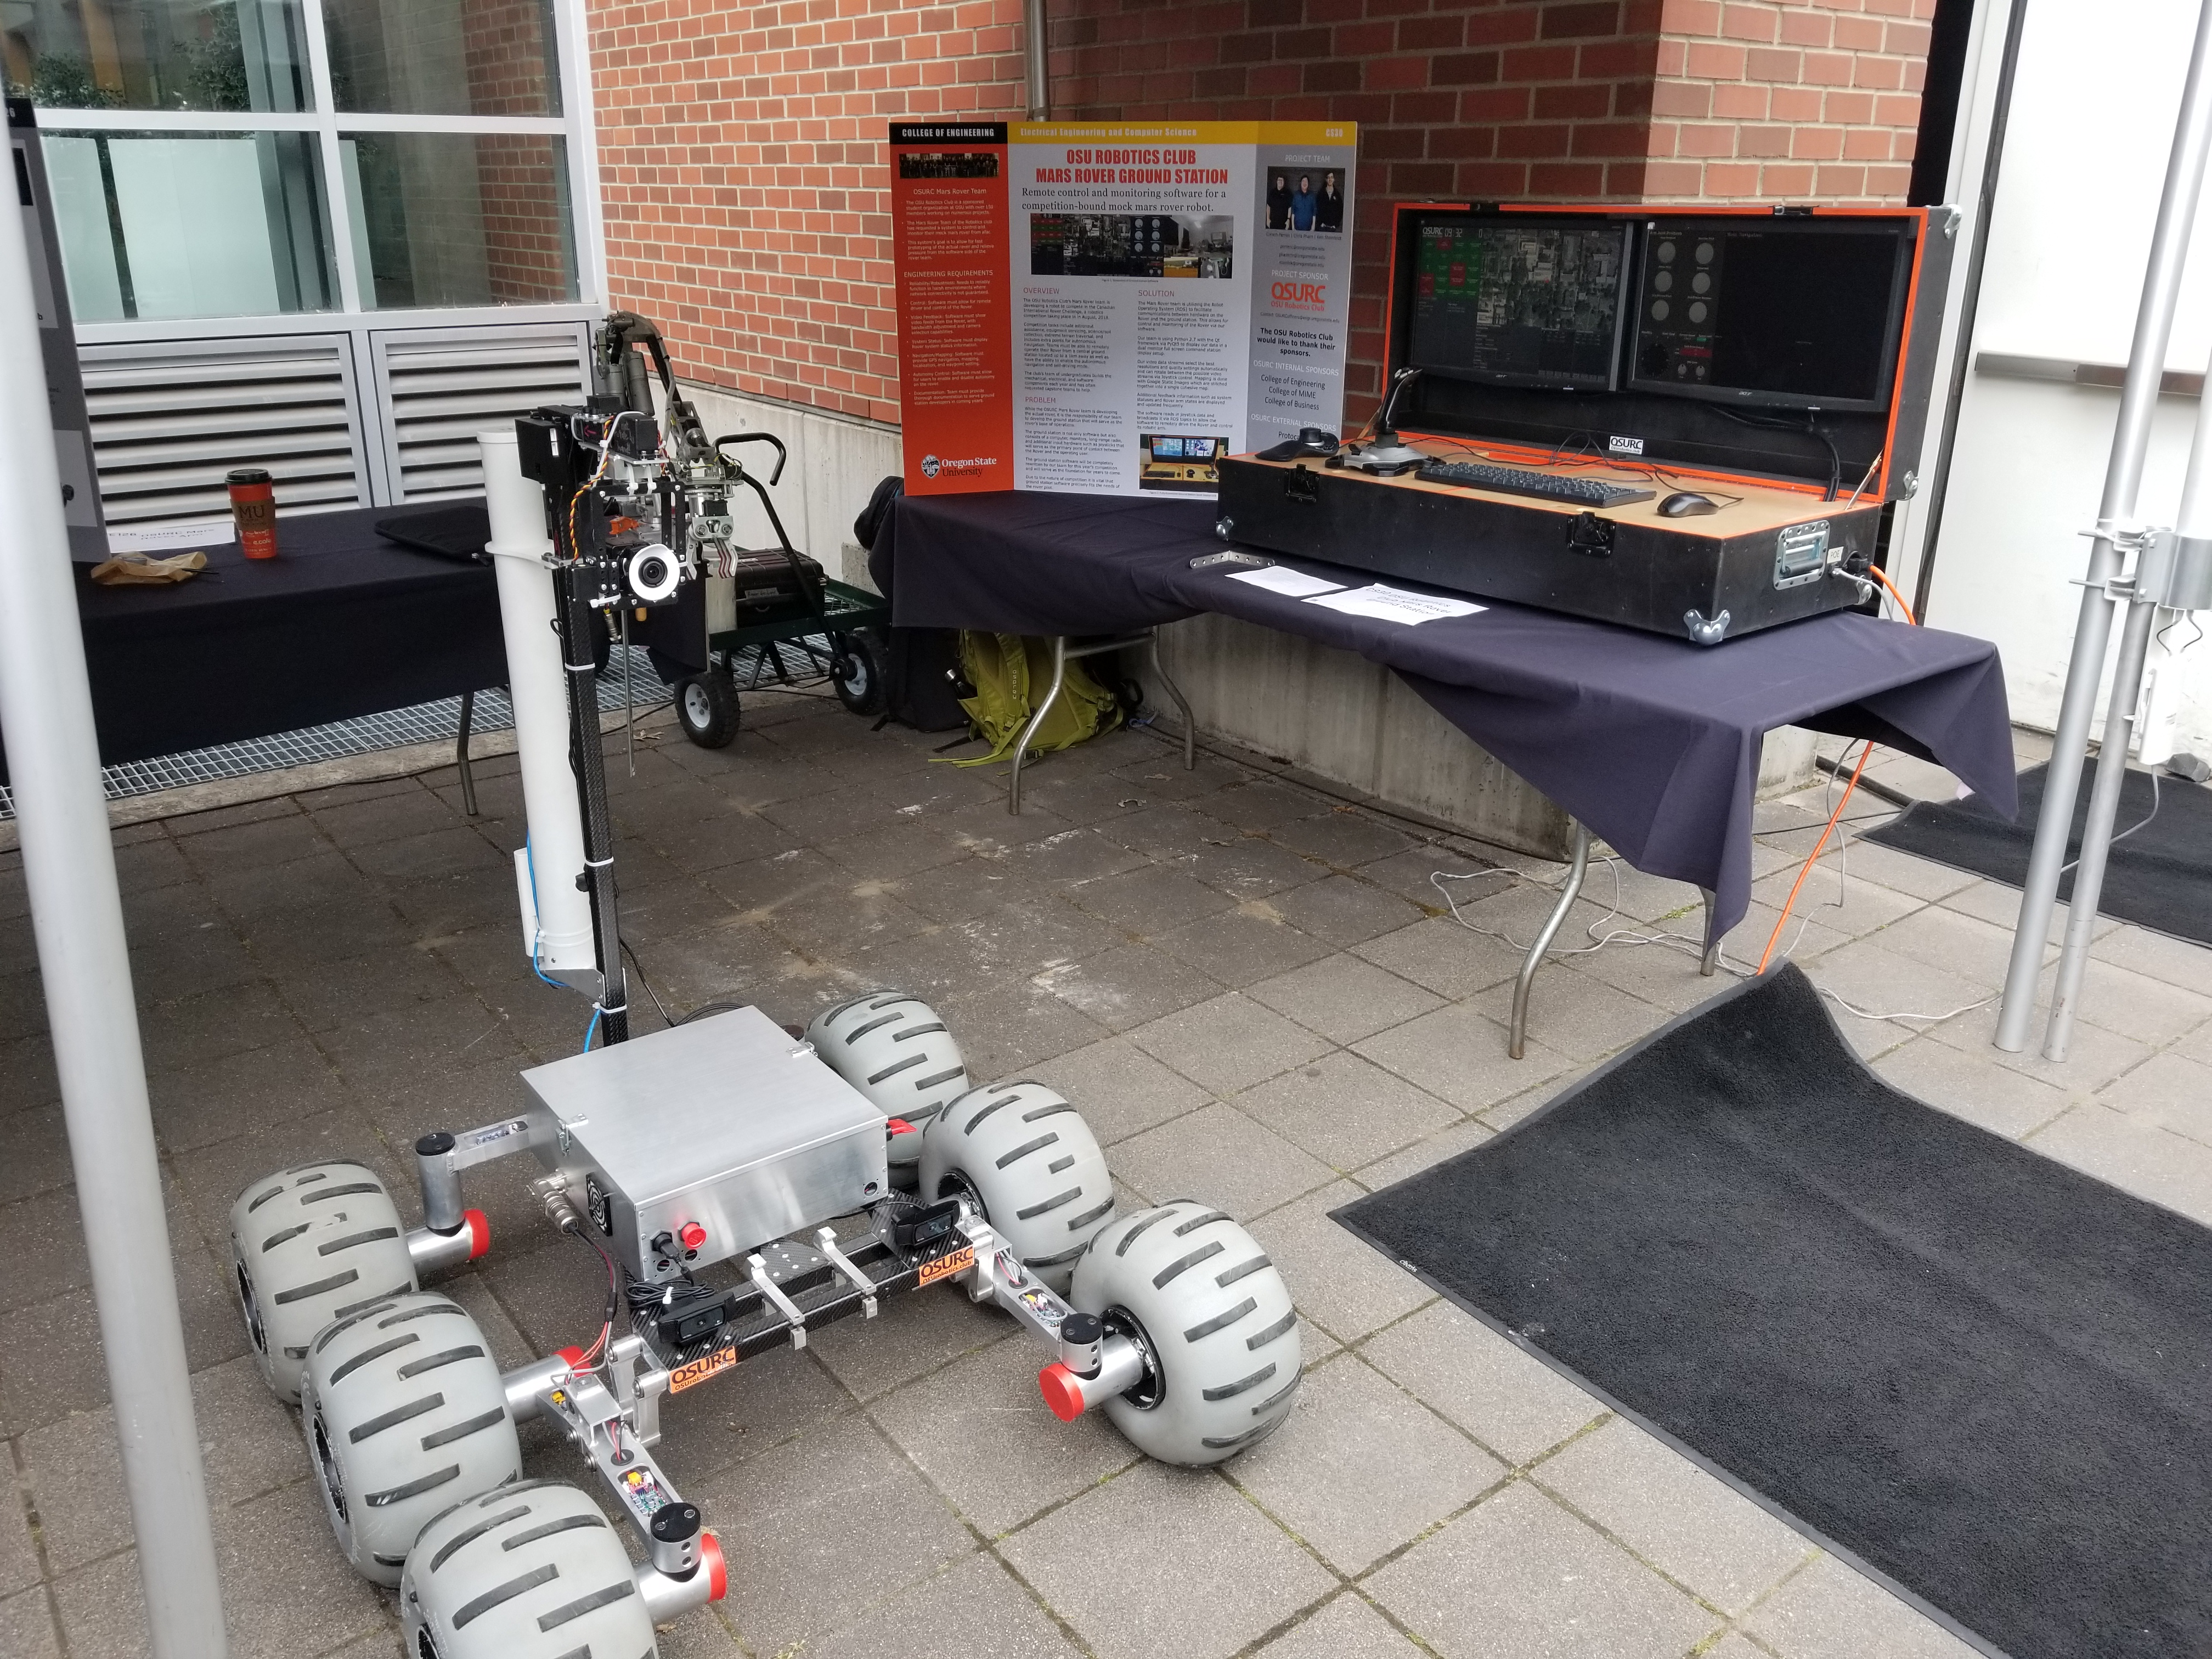
\includegraphics[width=0.9\textwidth]{misc_media/ground_station_expo}
  \caption{Finished Ground Station at Expo}
\end{figure}

\begin{figure}[h!]
  \centering
  \captionsetup{justification=centering}
  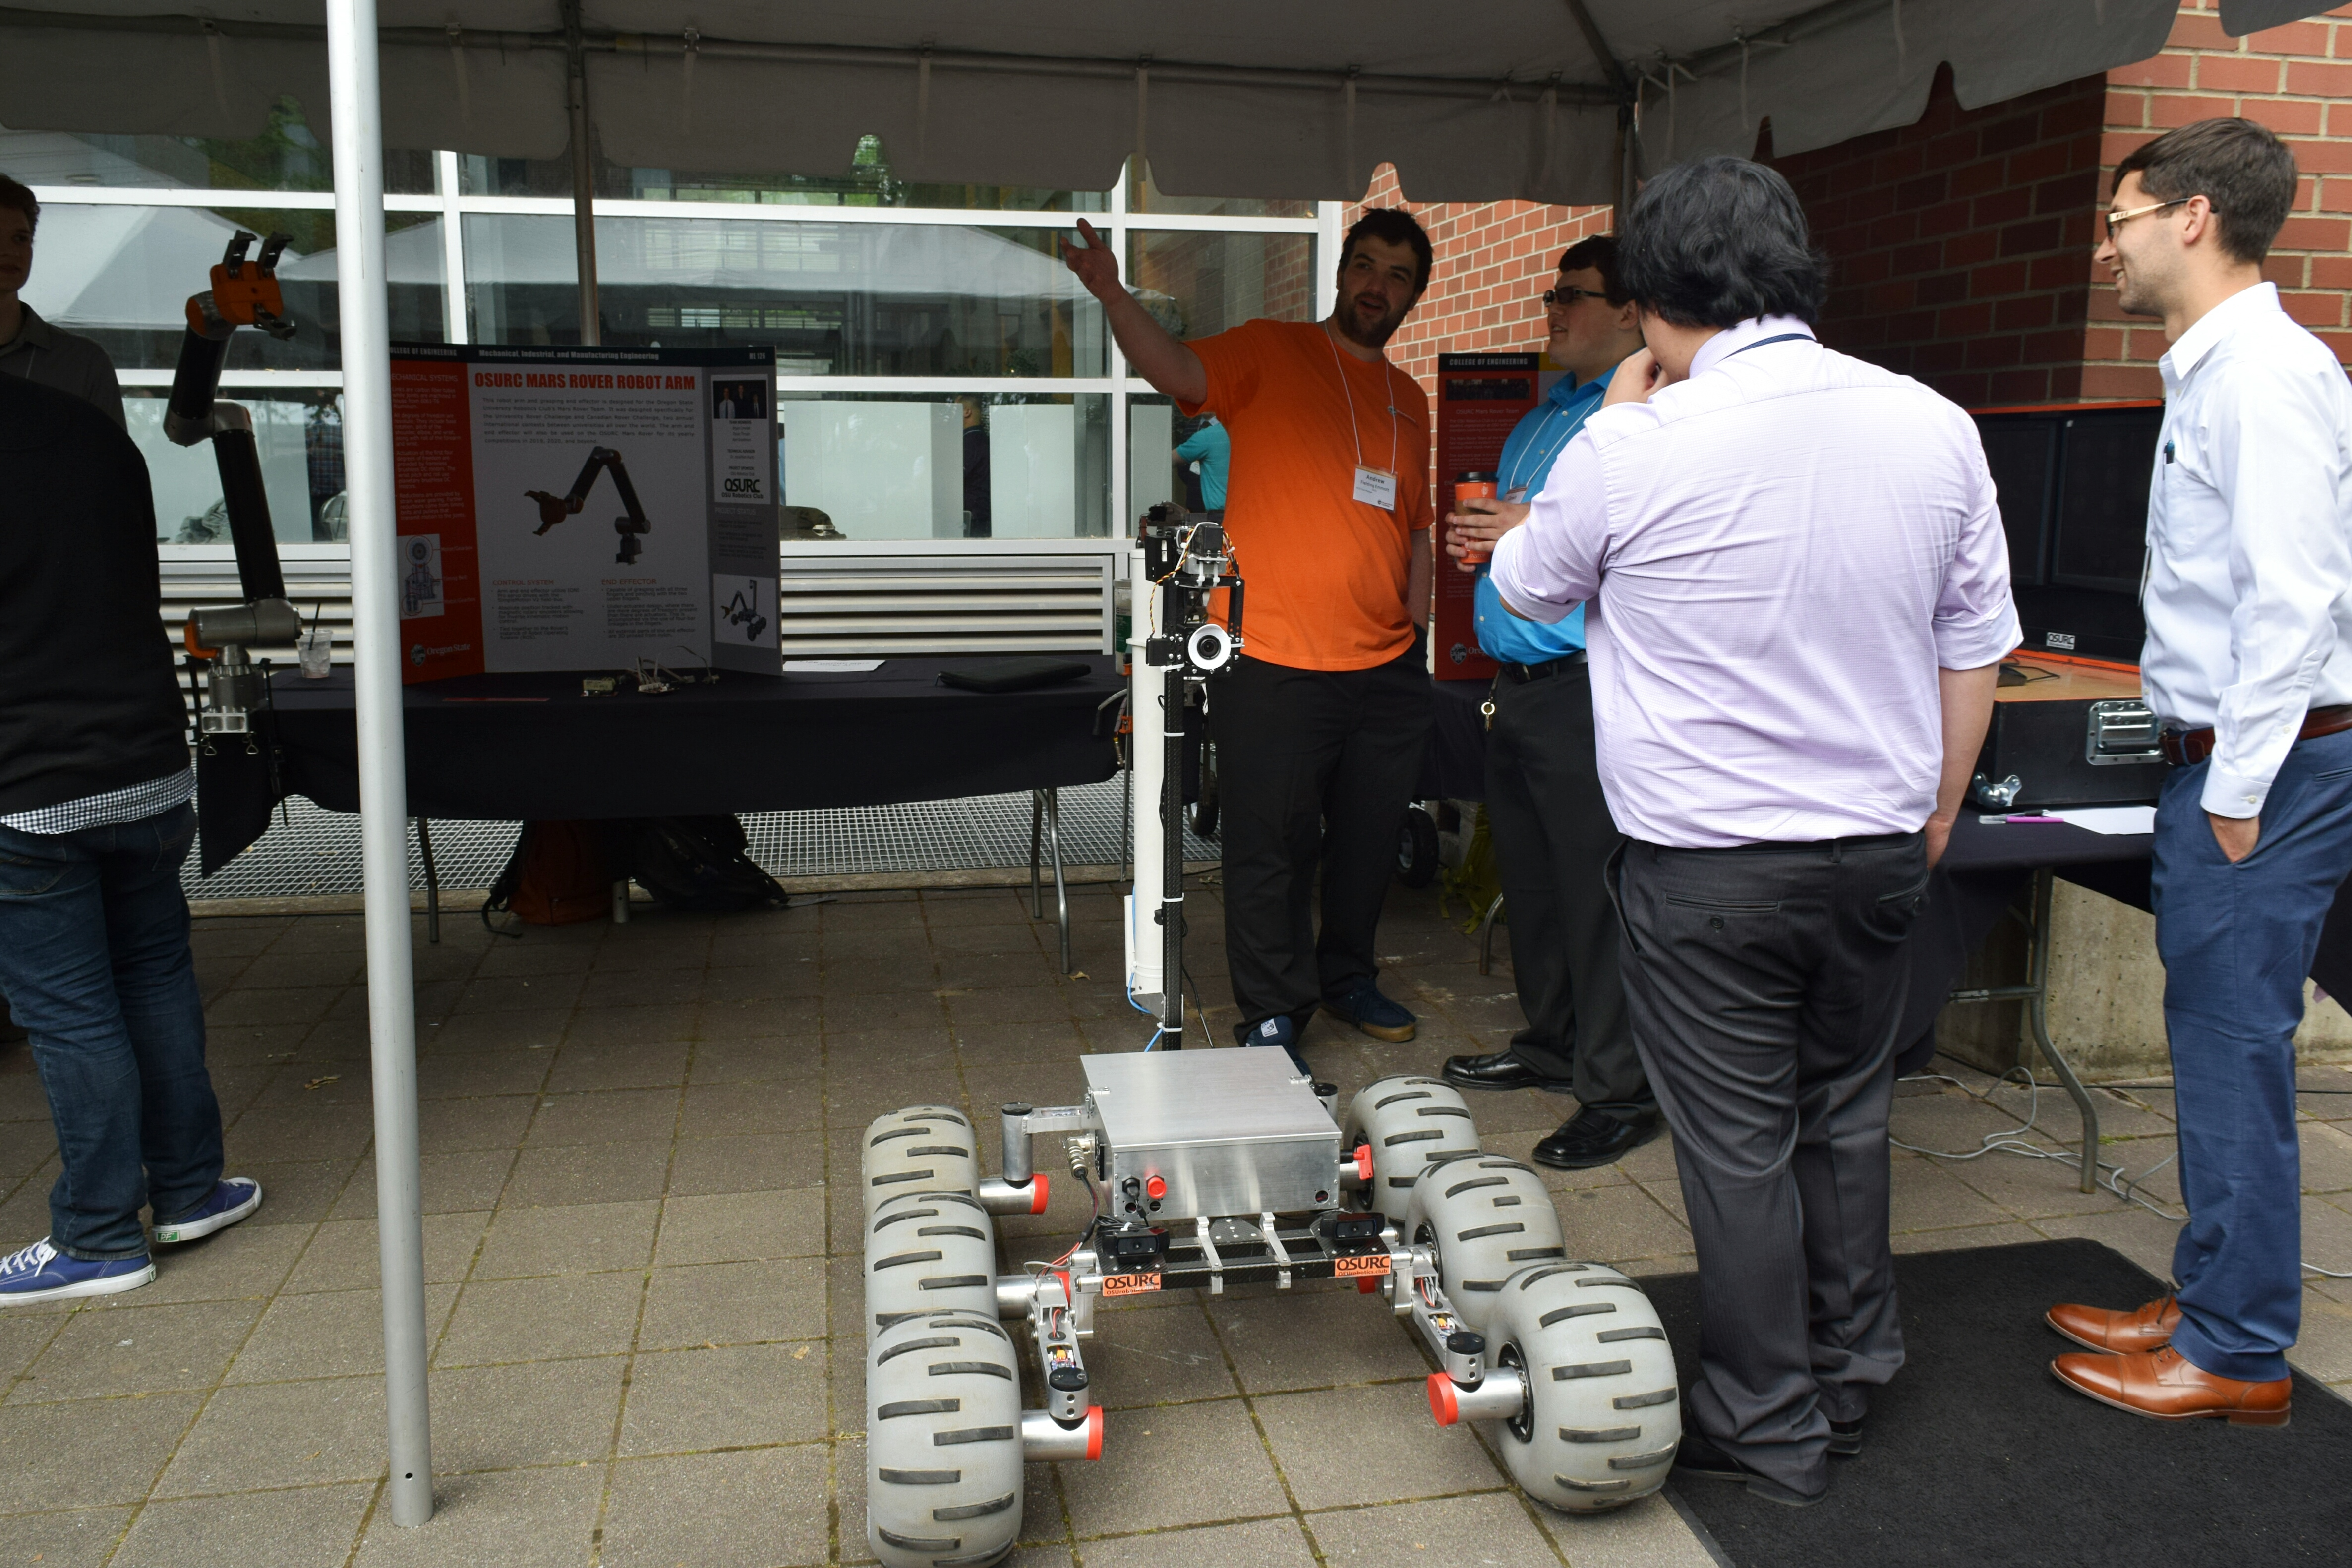
\includegraphics[width=0.9\textwidth]{misc_media/ground_station_expo_2}
  \caption{Chatting with TA at Expo}
\end{figure}
\end{document}





